\documentclass[10.75pt,a4paper,openright,bottom=2cm]{article}
\usepackage[english]{babel}
\usepackage[T1]{fontenc} 
\usepackage[utf8]{inputenc}
\usepackage{graphicx}
\usepackage{auto-pst-pdf} 
\usepackage{float}
\usepackage{graphicx}
\usepackage{wrapfig}
%\usepackage{subcaption}
\usepackage{textcomp}
\usepackage{geometry}
\usepackage{pdfpages}
\usepackage{amsmath}
\usepackage{amsfonts}
\usepackage{wrapfig}
\usepackage{lipsum} 
\usepackage{fancyhdr}
\usepackage{amsmath}
\usepackage{graphicx}
\usepackage[most]{tcolorbox}
\usepackage{bbm}
\usepackage{braket}
\usepackage{amssymb}
\usepackage{pifont}
\newcommand{\cmark}{\ding{51}}%
\newcommand{\xmark}{\ding{55}}%
\usepackage[table]{xcolor, colortbl}
\usepackage{cancel}
\DeclareMathAlphabet{\pazocal}{OMS}{zplm}{m}{n}
\usepackage[colorlinks=true, allcolors=blue]{hyperref}
\usepackage{multicol}
\usepackage{physics}
\usepackage[super]{nth}
\usepackage{bbm}
\usepackage{tikz}
%\usepackage[compat=1.1.0]{tikz-feynman}
\usetikzlibrary{positioning}
\usepackage{circuitikz}
\usetikzlibrary{arrows,shapes,positioning}
\usetikzlibrary {arrows.meta} 
\usetikzlibrary{angles,quotes}
\usepackage{subfig}
\usepackage{mathtools}
\usepackage{amsmath}
\usepackage{amssymb}
\usepackage{amsthm}
\renewcommand{\Vec}[1]{\boldsymbol{#1}}
\renewcommand{\refeq}[1]{\hyperref[#1]{Equation (\ref{#1})}}
\newcommand{\RN}[1]{%
  \textup{\uppercase\expandafter{\romannumeral#1}}%
}
\newtcolorbox{mybox}{
    arc=0pt,width=\textwidth,colback={blue!30},boxrule=0pt,frame hidden
}
%\begin{tcolorbox}[arc=0pt,width=\textwidth,colback={blue!30},boxrule=0pt,frame hidden]
\title{\textbf{Condensed Matter :(}}
\author{Matteo D'Errigo}

\begin{document}
\maketitle
\tableofcontents
% \begin{abstract}
% \end{abstract}
\newpage
\section{Crystal Lattices}
A \textbf{crystal} is a periodic arrangement of atoms, a \textbf{Bravais lattice} (or crystal lattice) specifies the periodic array in which the repeated units of the crystal are arranged. These units may be single atoms, molecules, ions and so on but the Bravais lattice summarizes only the geometry of the underlying periodic structure, regardless of what the actual units are. There are two equivalent definitions:
\begin{mybox}
\textbf{Bravais Lattice {\color{blue!30}{g}}}
\hrule
\begin{enumerate}
    \item A Bravais lattice is an infinite array of discrete points with an arrangement and orientation that appears \textbf{exactly} the same from whichever of the points the array is viewed
    \item A (3D) Bravais lattice is defined as a regular periodic arrangements of points in space, all of them connected by translation vectors $\Vec{R}$ of the form:
    \[
    \Vec{R}=n_1\Vec{a_1}+n_2\Vec{a_2}+n_3\Vec{a_3}
    \]
    where $\Vec{a_1}, \Vec{a_2}$ and $\Vec{a_3}$ are any three vectors not all in the same plane, $n_1, n_2$ and $n_3$ range through all integer values.
\end{enumerate}
\end{mybox}
\noindent
The vectors $\Vec{a_i}$ are called \textbf{primitive vectors} and they generate or span the lattice. The two definitions are equivalent, any array satisfying 1. satisfies 2. as well.\\
A volume of space that, when translated through all the vectors in a Bravais lattice, just fills all of space without either overlapping itself or leaving voids is called a \textbf{primitive unit cell}, with volume $\Omega=\Vec{a_1}\cdot(\Vec{a_2}\times\Vec{a_3})$.\\
The choice of primitive translation vectors, hence the shape of the primitive cell, is not unique, only the volume of the unit cell is invariant. A primitive cell must contain exactly one lattice point: it follows that if $n$ is the density of points in the lattice and $V$ is the volume of the cell, then $nV=1$. Therefore, $V=1/n$ and this result holds true for any primitive cell.\\
The obvious primitive cell to associate with a particular set of primitive vectors $\{\Vec{a_1},\Vec{a_2},\Vec{a_3}\}$ is the set of all points $\Vec{r}$ of the form:
\[
\Vec{r}=x_1\Vec{a_1}+x_2\Vec{a_2}+x_3\Vec{a_3}
\]
for $x_i$ ranging continuously between 0 and 1. This choice has the disadvantage of not displaying the full symmetry of the lattice. It is important to work with cells that have the full symmetry of their lattice and there are two solutions to this problem:
\begin{itemize}
    \item \textbf{Conventional unit cell}: one can fill up space with non-primitive unit cells, the conventional unit cell is generally chosen to be bigger than the primitive cell and to have the required symmetry
    \item \textbf{Wigner-Seitz primitive cell}: one can choose a primitive cell with the full symmetry of the lattice. The most common choice is the Wigner-Seitz cell which is defined as the region of space that is closer to a specific point than to any other lattice point. Since there is nothing in this definition that refers to any particular choice of primitive vectors, the Wigner-Seitz cell will be as symmetrical as the Bravais lattice. Since any lattice point has a unique lattice point as its nearest neighbour it will belong to exactly one Wigner-Seitz cell. Translating the Wigner-Seitz cell through all the lattice vectors will just fill the space without overlapping, hence the Wigner-Seitz cell is primitive.
\end{itemize}
\newpage
\noindent
\textbf{Examples of Cubic Lattices}\\\\
\begin{wrapfigure}{r}{0.45\textwidth}
    \vspace{-0.75cm}
    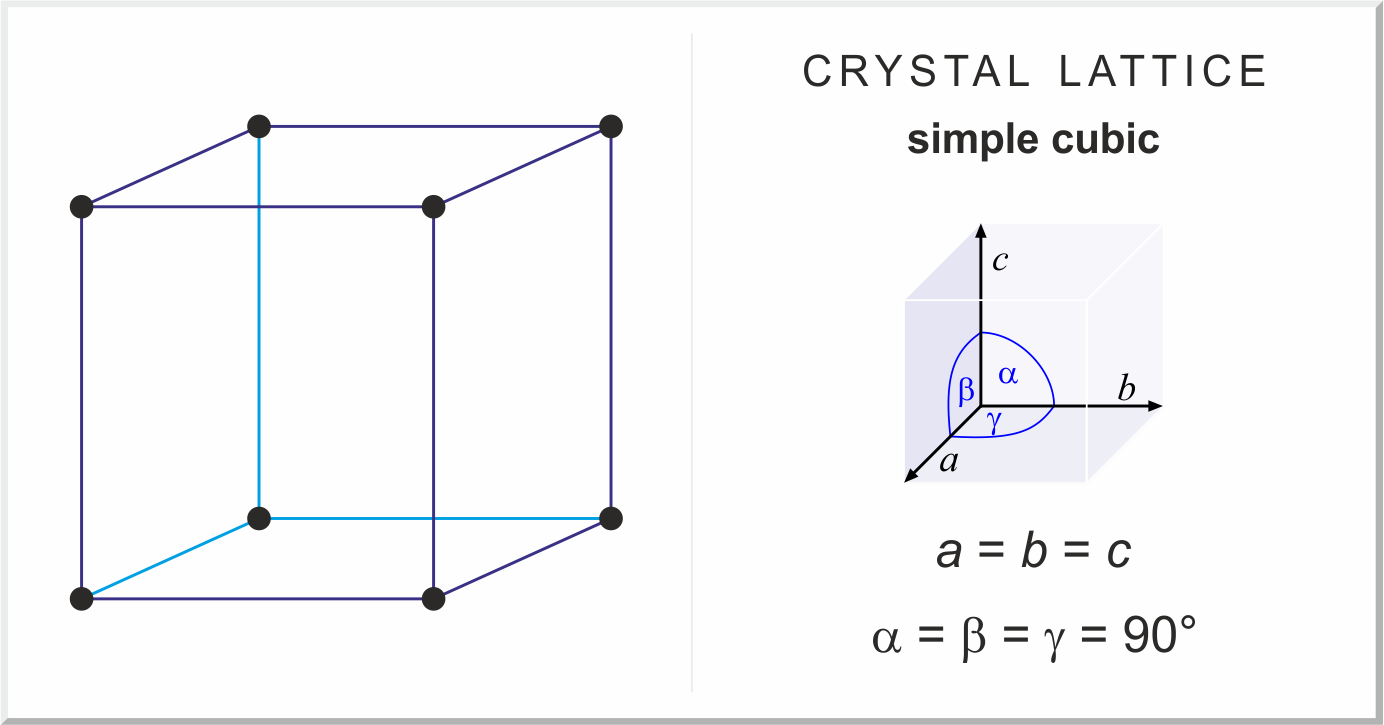
\includegraphics[width=0.45\textwidth]{simple_cubic_lattice.png}
    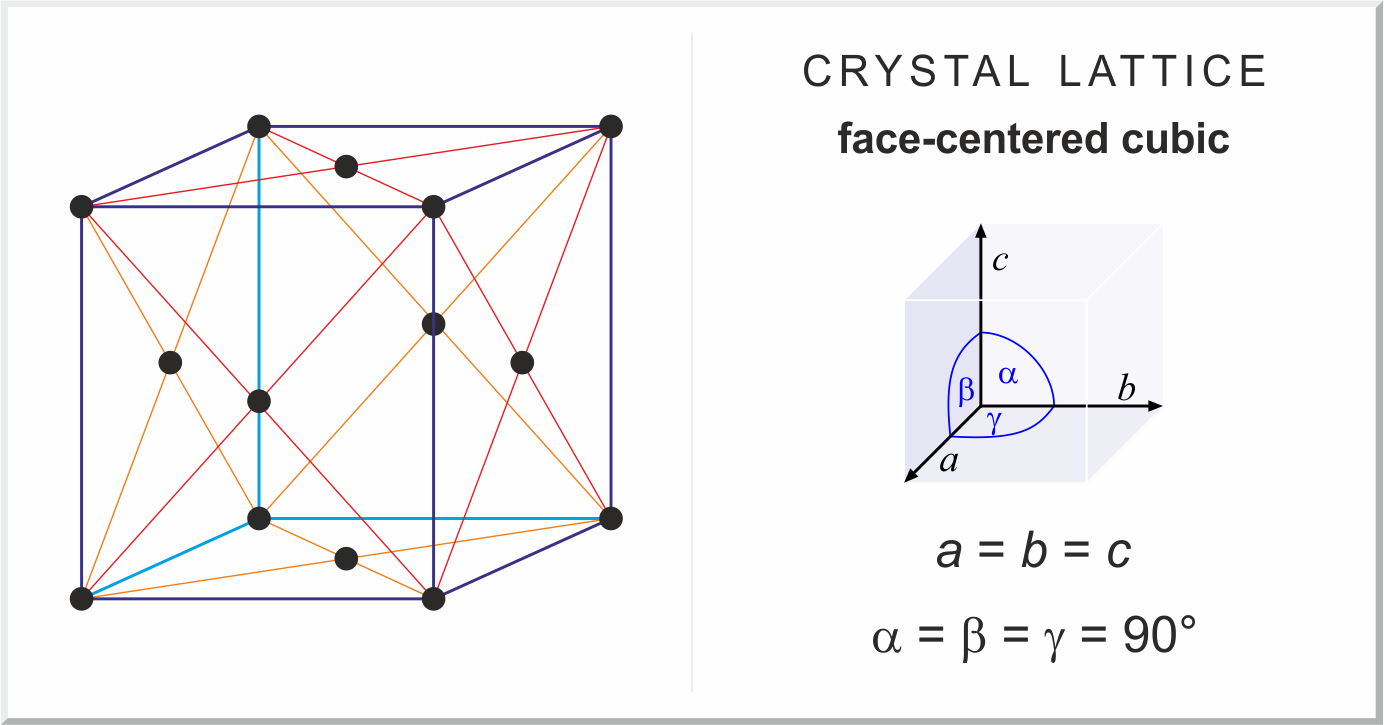
\includegraphics[width=0.45\textwidth]{face-centered_cubic_lattice.png}
    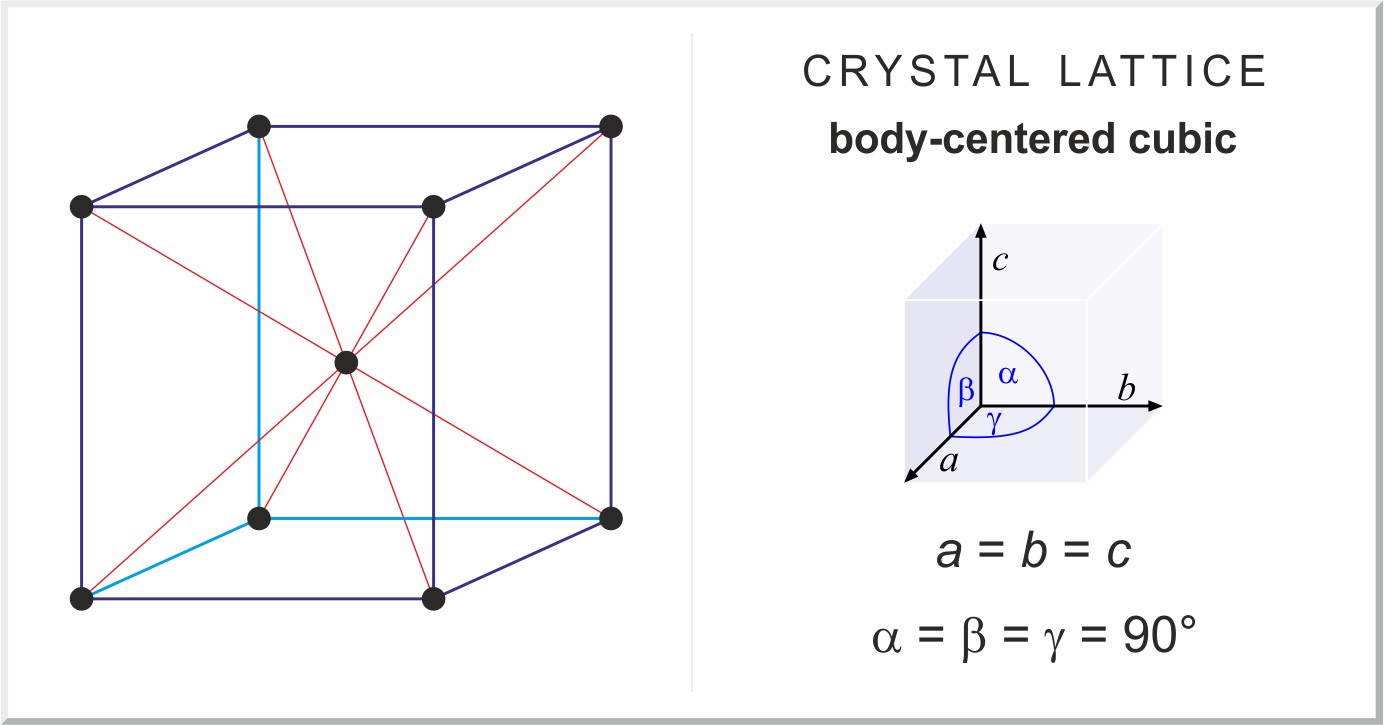
\includegraphics[width=0.45\textwidth]{body-centered_cubic_lattice.png}
    \end{wrapfigure}
    $\bullet$\;\textbf{Simple cubic} (SC): it can be spanned by three mutually perpendicular primitive vectors of equal length
    \[
    \Vec{t_1}=a(1,0,0) \quad \Vec{t_2}=a(0,1,0) \quad \Vec{
    t_3}=a(0,0,1)
    \]\\\\\\
    $\bullet$\;\textbf{Face-centered cubic} (FCC): it is constructed by adding to the SC an additional point in the center of each square face. A symmetric set of primitive vectors for the FCC is:
    \[
    \Vec{t_1}=\frac{a}{2}(0,1,1) \quad \Vec{t_2}=\frac{a}{2}(1,0,1) \quad \Vec{t_3}=\frac{a}{2}(1,1,0)
    \]\\\\\\
    $\bullet$\;\textbf{Body-centered cubic} (BCC): it is formed by adding to the SC an additional point at the center of each little cube.
    \[
    \Vec{t_1}=\frac{a}{2}(-1,1,1) \quad \Vec{t_2}=\frac{a}{2}(1,-1,1) \quad \Vec{t_3}=\frac{a}{2}(1,1,-1)
    \]
\newline
\subsection{The Reciprocal Lattice}
Consider a set of points $\Vec{R}$ constituting a Bravais lattice and a plane wave $e^{i\Vec{k}\cdot\Vec{r}}$ traveling through a crystal. For general $\Vec{k}$ such plan wave will not have the periodicity of the Bravais lattice but it will for certain special choices: let $\Vec{k}=\Vec{G}$ a \textit{particular} wave vector that makes the wave have the same periodicity of the lattice.
\begin{mybox}
\textbf{Reciprocal Lattice}
\hrule
\vspace{0.15cm}
The set of all wave vectors $\Vec{G}$ that yield plane waves with the periodicity of a given Bravais lattice is known as its \textbf{reciprocal lattice}. This is true if:
\[
e^{i\Vec{G}\cdot(\Vec{r}+\Vec{R})}=e^{i\Vec{G}\cdot\Vec{r}}\xleftrightarrow{}e^{i\Vec{G}\cdot\Vec{R}}=1\Rightarrow\Vec{G}\cdot\Vec{R}=2\pi m\,,\;m\in\mathbb{Z}
\]
for all $\Vec{R}$ in the Bravais lattice. Note that a reciprocal lattice is defined with reference to a particular Bravais lattice, referred as the direct lattice.
\end{mybox}
\noindent
Take now $\Vec{R}=n_1\Vec{a_1}+n_2\Vec{a_2}+n_3\Vec{a_3}$ and $\Vec{G}=m_1\Vec{b_1}+m_2\Vec{b_2}+m_3\Vec{b_3}$. The condition found above is telling us that:
\[
\Vec{G}\cdot\Vec{R}=2\pi m=n_1m_1\Vec{b_1}\cdot\Vec{a_1}+n_2m_2\Vec{b_2}\cdot\Vec{a_2}+n_3m_3\Vec{b_3}\cdot\Vec{a_3}
\]
The three primitive vectors $\{\Vec{b_1},\Vec{b_2},\Vec{b_3}\}$ generating the reciprocal lattice are chosen to be:
\[
\Vec{b_1}=2\pi\frac{\Vec{a_2}\times\Vec{a_3}}{\Vec{a_1}\cdot(\Vec{a_2}\times\Vec{a_3})} \quad
\Vec{b_2}=2\pi\frac{\Vec{a_3}\times\Vec{a_1}}{\Vec{a_1}\cdot(\Vec{a_2}\times\Vec{a_3})}\quad
\Vec{b_3}=2\pi\frac{\Vec{a_1}\times\Vec{a_2}}{\Vec{a_1}\cdot(\Vec{a_2}\times\Vec{a_3})}\quad
\]
To verify this, note that the vectors $\Vec{b_i}$ satisfy $\Vec{b_i}\cdot\Vec{a_j}=2\pi\delta_{ij}$. With this choice of primitive vectors for the reciprocal lattice, we then have:
\[
\Vec{G}\cdot\Vec{R}=2\pi(n_1m_1+n_2m_2+n_3m_3)
\]
For $e^{i\Vec{G}\cdot\Vec{R}}$ to be equal to 1 for all $\Vec{R}$, $\Vec{G}\cdot\Vec{R}$ must be $2\pi m$ for $m$ integer for any choices of integers $n_i$. This requires $m_i$ to be integers as well: $\Vec{G}$ is then a reciprocal lattice vector for those vectors that are linear combinations of the $\Vec{b_i}$ for integer coefficients. It follows that the reciprocal lattice is a Bravais lattice and $\Vec{b_i}$ can be taken as primitive vectors.\\
Take now a function $u(\Vec{r})$ which satisfies $u(\Vec{r}+\Vec{R})=u(\Vec{r})$ for any $\Vec{R}$ Bravais lattice vector and compute its Fourier transform, i.e. expand it in plane waves:
\[
u(\Vec{r})=\sum_{\Vec{k}}u_{\Vec{k}}e^{i\Vec{k}\cdot\Vec{r}}
\]
By means of the periodicity condition, the space of $\Vec{k}$ can be restricted to the set corresponding to the reciprocal space.
\[
u(\Vec{r})=\sum_{\Vec{G}}u_{\Vec{G}}e^{i\Vec{G}\cdot\Vec{r}} \quad u_{\Vec{G}}:=\frac{1}{V_c}\int d\Vec{r}u(\Vec{r})e^{-i\Vec{G}\cdot\Vec{r}}
\]
where $V_c$ is the volume of a primitive unit cell. Explicitly computing $u_{\Vec{G}}$ gives us:
\[
u_{\Vec{G}}=\frac{1}{V_c}\int d\Vec{r}\sum_{\Vec{G'}}u_{\Vec{G'}}e^{i\Vec{G'}\cdot\Vec{r}}e^{-i\Vec{G}\cdot\Vec{r}}=\frac{1}{V_c}\sum_{\Vec{G'}}\int d\Vec{r}u_{\Vec{G'}}e^{i(\Vec{G'}-\Vec{G})\cdot\Vec{r}}=u_{\Vec{G'}}\delta(\Vec{G}-\Vec{G'})
\]
The reciprocal lattice can be seen as the Fourier transform of the direct lattice. Consider now the 1D case where $u(r)=\rho(r)$, defined as:
\[
\rho(r)=\sum_{n\in\mathbb{Z}}\delta(r-na)
\]
which corresponds to the density of points in the direct space of a 1D crystal lattice. Take its Fourier transform:
\[
\text{FT}[\rho(r)]=\int_{\mathbb{R}}dre^{ikr}\rho(r)=\sum_{n\in\mathbb{Z}}\int_\mathbb{R}dre^{ikr}\delta(r-na)=\sum_{n\in\mathbb{Z}}e^{ikna}=\frac{2\pi}{a}\sum_{m\in\mathbb{Z}}\delta\left(k-\frac{2\pi m}{a}\right)
\]
This result can be generalized to any dimension $D$:
\[
\rho(\Vec{r})=\sum_{\Vec{R}}\delta(\Vec{r}-\Vec{R})\Rightarrow\text{FT}[\rho(\Vec{r}]=\frac{(2\pi)^D}{a^D}\sum_{\Vec{G}}\delta^D(\Vec{k}-\Vec{G})
\]
\newpage
\subsection{Lattice Planes}
There is a relation between vectors in the reciprocal lattice and planes of points in the direct lattice, which is important in understanding the role of the reciprocal lattice in diffraction theory.\\
Given a particular Bravais lattice, a \textbf{lattice plane} is defined to be any plane containing at least three non-collinear Bravais lattice points. A \textbf{family of lattice planes} is a set of parallel equally spaced lattice planes which together contain all the points of the 3D Bravais lattice. The resolution of a Bravais lattice into a family of lattice planes is not unique.
\begin{figure}[h!]
    \centering
    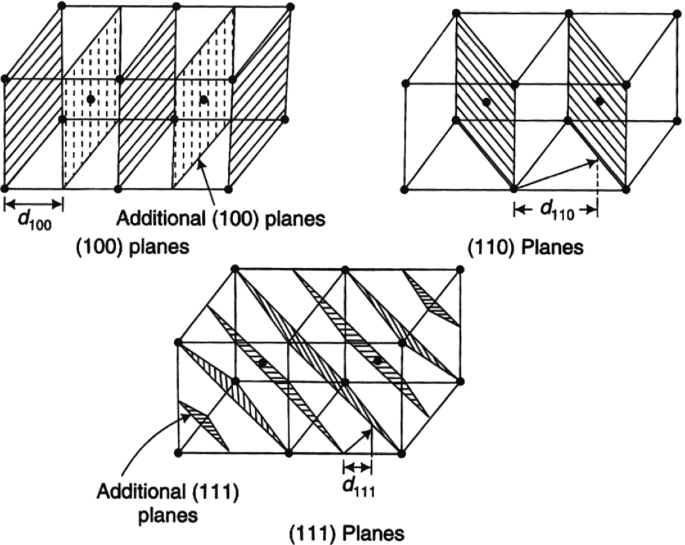
\includegraphics[width=0.6\textwidth]{lattice_planes.png}
     
    \label{fig:lattice_planes}
\end{figure}\\
\noindent
The reciprocal lattice provides a simple way to classify all possible families of lattice planes, summarized in the following theorem.
\begin{mybox}
\textbf{Family of Lattice Planes}
\hrule
\vspace{0.15cm}
For any family of lattice planes separated by a distance $d$, there are reciprocal lattice vectors perpendicular to the planes, the shortest of which have a length of $2\pi/d$.\\
Conversely, for any reciprocal lattice vector $\Vec{G}$ there is a family of lattice planes normal to $\Vec{G}$ and separated by a distance $d$, where $2\pi/d$ is the length of the shortest reciprocal lattice vector parallel to $\Vec{G}$.
\end{mybox}
\noindent
The correspondence between reciprocal lattice vectors and families of lattice planes provides a convenient way to specify the orientation of a lattice plane. Generally, one describes the orientation of a plane by giving a vector normal to the plane. Since we know there are reciprocal lattice vectors normal to any family of lattice planes, it is natural to pick a reciprocal lattice vector to represent the normal. To make the choice unique, one uses the shortest one, arriving at the \textbf{Miller indices} of the plane.
\begin{mybox}
\textbf{Miller Indices {\color{blue!30}{g}}}
\hrule
\vspace{0.15cm}
The Miller indices of a lattice plane are the coordinates of the shortest reciprocal lattice vector normal to that plane, with respect to a specified set of primitive reciprocal lattice vectors. A plane with Miller indices $h,k,l$ is normal to the reciprocal lattice vector identified by $h\Vec{b_1}+k\Vec{b_2}+l\Vec{b_3}$.
\end{mybox}
\noindent
The Miller indices are integers, since any reciprocal lattice vector is a linear combination of three primitive vectors with integer coefficients. Because the normal to the plane is specified by the shortest perpendicular reciprocal lattice vector, the integers $h,k,l$ can have no common factor.
\begin{mybox}
\textbf{Miller Indices Conventions {\color{blue!30}{g}}}
\hrule
\vspace{0.15cm}
Lattice planes are specified by giving the Miller indices in parentheses $(h,k,l)$. Commas are eliminated by writing $\overline{n}$ instead of $-n$. To specify directions in the direct lattice, but to avoid confusion, square brackets are used instead of parentheses. The $(100), (010)$ and $(001)$ planes are all equivalent in a cubic crystal, they are referred collectively as the $\{100\}$ planes. Similarly for the directions, one write $\Braket{100}$.
\end{mybox}
\noindent
\begin{wrapfigure}{r}{0.4\textwidth}
    \centering
    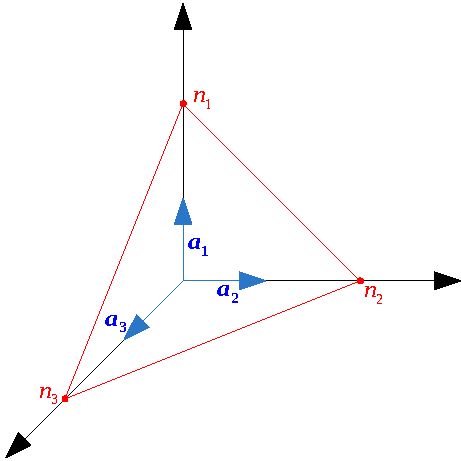
\includegraphics{miller.pdf}
    \centering
    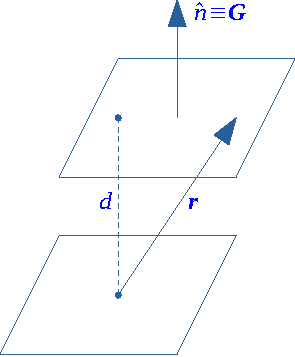
\includegraphics{d.pdf}
\end{wrapfigure}
By definition, the reciprocal lattice vector identified by $\Vec{G}=h\Vec{b_1}+k\Vec{b_2}+l\Vec{b_3}$ has to be orthogonal to the generic plane displayed in the top picture on the side. This is possible if:
\[
\Vec{G}\cdot(n_1\Vec{a_1}-n_2\Vec{a_2})=\Vec{G}\cdot(n_1\Vec{a_1}-n_3\Vec{a_3})=\Vec{G}\cdot(n_2\Vec{a_2}-n_3\Vec{a_3})=0
\]
By using the fact that $\Vec{a_i}\cdot\Vec{b_j}=2\pi\delta_{ij}$, we get:
\[
hn_1-kn_2=hn_1-ln_3=kn_2-ln_3=0
\]
A possible solution is therefore:
\[
h=\frac{1}{n_1} \qquad k=\frac{1}{n_2} \qquad l=\frac{1}{n_3}
\]
The physical interpretation of the Miller indices is that they give the right weight in the linear combination of primitive reciprocal vectors to obtain $\Vec{G}$.\\
Miller indices are also used to determine the relation between the distance between lattice planes $d$ and the distance between lattice points $a$. Look at the bottom picture on the side: the translation vector $\Vec{r}$ can be chosen arbitrarily on the plane, e.g. $\Vec{r}=n_1\Vec{a_1}$. The distance between the two planes is given by:
\[
d=\Vec{r}\cdot\hat{n}=n_1\Vec{a_1}\frac{\Vec{G}}{|\Vec{G}|}=n_1\Vec{a_1}\frac{h\Vec{b_1}+k\Vec{b_2}+l\Vec{b_3}}{|\Vec{G}|}
\]
Remembering that $\Vec{a_i}\cdot\Vec{b_j}=2\pi\delta_{ij}$ and that $h=1/n_1$, we then have:
\[
d=2\pi\frac{n_1h}{|\Vec{G}|}\Rightarrow|\Vec{G}|=\frac{2\pi}{d}
\]
For a cubic lattice, we can establish another important relation, being $\Vec{G}=\frac{2\pi}{a}(h,k,l)$:
\[
d=n_1a(1,0,0)\frac{\frac{2\pi}{a}(h,k,l)}{\frac{2\pi}{a}\sqrt{h^2+k^2+l^2}}\underset{\mathclap{\tikz \node {$\uparrow$} node [below=1ex] {\footnotesize $h=\frac{1}{n_1}$};}}{=}\frac{a}{\sqrt{h^2+k^2+l^2}}
\]
% \begin{wrapfigure}{l}{0.45\textwidth}
%     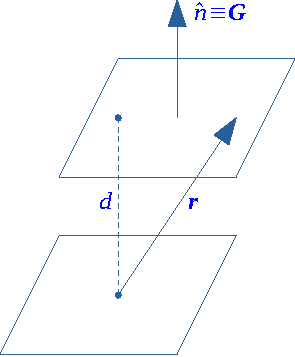
\includegraphics{d.pdf}
% \end{wrapfigure}

\newpage
\section{Diffraction}
When waves propagates through a crystal with wavelength of the same order of the primitive cell dimensions, there will be the phenomenon of \textbf{diffraction}. Different type of waves can propagates through the crystal:
\begin{itemize}
    \item Electromagnetic waves (X-rays)
    \item Charged particles (electrons)
    \item Neutral particles (neutrons)
\end{itemize}
For X-rays, diffraction is caused by the electrons in the crystal, for charged particles it is due to electrons and nuclei while for neutral particles is produced essentially by the nuclei in the crystal.\\
Typical interatomic distances in a solid are on the order of an angstrom $(10^{-8}$\,cm). An electromagnetic probe of the microscopic structure must have a wavelength at least this short, corresponding to an energy of $\sim10^3$\,eV: these are characteristic X-ray energies.
\begin{figure}[h]
    \centering
    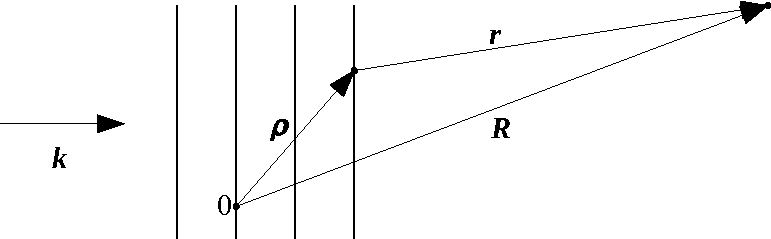
\includegraphics{diffraction.pdf}
     
    \label{fig:diffraction}
\end{figure}\\
In every scattering phenomenon from a point $\Vec{\rho}$, the amplitude of the diffused wave in the point identified by $\Vec{r}$ is proportional to the amplitude of the incoming wave in the scattering point (which can be approximated as a plane wave being the source far away) and to the amplitude of the outgoing spherical wave:
\[
\text{Incoming plane wave:}\;\; F_0e^{i\Vec{k}\cdot\Vec{\rho}} \qquad \text{Outgoing spherical wave:}\;\; D\frac{e^{i\Vec{k'}\cdot\Vec{r}}}{\Vec{r}}
\]
In the case X-rays are used, the points $\Vec{\rho}$ indicate the position of all the electrons in the crystal, which are the only scattering centers being much lighter than the nuclei. The proportional factor $D$ is given by:
\[
D=\frac{e^2}{mc^2}\sqrt{\frac{1+\cos^2\phi}{2}}
\]
where $\phi$ is the incident angle between the incoming direction and the diffusion one.\\
Scattering from different centers in different points gives place to interference which will be constructive only in specific directions, depending on the crystal periodicity and the wavelength. Consider now the scattering of plane waves from a crystal point $\Vec{\rho}$ towards an external point defined by $\Vec{R}$ from the origin. Using the following approximations:
\[
\Vec{R}=\Vec{r}+\Vec{\rho} \quad \Vec{R},\Vec{r}\gg\Vec{\rho} \quad \Vec{r}\simeq\Vec{R}-\Vec{\rho}\cos\theta
\]
the amplitude of the scattered wave then becomes:
\[
A\propto\frac{e^{i\Vec{k}\cdot\Vec{\rho}}e^{i\Vec{k'}\cdot(\Vec{R}-\Vec{\rho}\cos\theta)}}{\Vec{R}}
\]
The factor $e^{i\Vec{k'}\cdot\Vec{R}}$ does not depend on the diffusion point, hence it can be treated as a constant. The factor $e^{-i\Vec{k'}\Vec{\rho}\cos\theta}$ can be written as:
\[
e^{-i\Vec{k'}\Vec{\rho}\cos\theta}\simeq e^{-i\Vec{k'}\Vec{\rho}\frac{\Vec{R}}{|\Vec{R}|}}\approx e^{-i\Vec{k'}\Vec{\rho}\cdot\Vec{\hat{r}}}=e^{-i\Vec{k'}\cdot\Vec{\rho}}
\]
$\Vec{k'}$ defines the direction of the scattered wave. It follows that we have an amplitude of the type:
\[
A\propto e^{i\Vec{k}\cdot\Vec{\rho}}e^{-i\Vec{k}'\cdot\Vec{\rho}}=e^{-i\Vec{\rho}\cdot(\Vec{k}'-\Vec{k})}=e^{-i\Vec{\rho}\cdot\Delta\Vec{k}} \qquad \Delta\Vec{k}=\Vec{k}'-\Vec{k}
\]
Considering all the terms we have:
\[
A=\frac{e^2}{mc^2}\sqrt{\frac{1+\cos^2\phi}{2}}\frac{F_0}{\Vec{R}}e^{i\Vec{k'}\cdot\Vec{R}}e^{-i\Vec{\rho}\cdot\Delta\Vec{k}}=C(\phi)e^{-i\Vec{\rho}\cdot\Delta\Vec{k}}
\]
The wave vector of the scattered wave $\Vec{k'}$ and the wave vector of the incoming wave $\Vec{k}$ must have equal modulus because we are considering elastic scattering.\\
If the points $\Vec{\rho}$ belong to a crystal lattice, it is possible to relate them to the points $\Vec{\rho_0}$ of the primitive cell:
\[
\Vec{\rho}=\Vec{\rho_0}+n_1\Vec{t_1}+n_2\Vec{t_2}+n_3\Vec{t_3}
\]
The relative total contribution will then be proportional to:
\begin{equation}
\label{rhozero}
e^{-i\Vec{\rho_0}\cdot\Delta\Vec{k}}\sum_{n_1n_2n_3}e^{-i(n_1\Vec{t_1}+n_2\Vec{t_2}+n_3\Vec{t_3})\cdot\Delta\Vec{k}}
\end{equation}
Summing over the translations will give e meaningful contribution only if the terms are equal to 1, i.e.:
\[
e^{-i\Vec{t_n}\cdot\Delta\Vec{k}}=1
\]
Using the definition of reciprocal lattice, this can be written as $\Delta\Vec{k}=\Vec{G}$ where $\Vec{G}$ is a generic vector of the reciprocal lattice. This is the \textbf{Laue law}.\\
It is possible to show that when the number of lattice points is large enough, there will be scattering of noticeable intensity only in the directions defined by the Laue condition. The scattered intensity is proportional to the product of three terms of the form:
\[
\left|\sum_{n=0}^{N-1}e^{-in\Vec{t}\cdot\Delta\Vec{k}}\right|^2=\left|\frac{1-e^{-iN\Vec{t}\cdot\Delta\Vec{k}}}{1-e^{-i\Vec{t}\cdot\Delta\Vec{k}}}\right|^2=\frac{\sin^2(N\Vec{t}\cdot\Delta\Vec{k}/2)}{\sin^2(\Vec{t}\cdot\Delta\Vec{k}/2)}
\]
Functions of this type are oscillating function of $\Vec{t}\cdot\Delta\Vec{k}$, with a maximum in $(2n+1)\pi/N$ and a minimum corresponding to zero in $2n\pi/N$. Taking into account the product of three factors of that type, the scattered intensity is different from zero only around those points where the function has a maximum value. The maximum intensity condition can be written as:
\[
\Vec{t_1}\cdot\Delta\Vec{k}=2\pi n \quad \Vec{t_2}\cdot\Delta\Vec{k}=2\pi m \quad \Vec{t_3}\cdot\Delta\Vec{k}=2\pi r
\]
where $n,m$ and $r$ are integer numbers. These are the Laue equations for lattice diffraction.\\
So far, we have not considered the structure of the primitive cell but only the effect of translation symmetry. To get the total amplitude, the contribution from \hyperref[rhozero]{Equation (\ref{rhozero})} have to be summed over all the points $\Vec{\rho}$ and take into account the density of scattering particles. In the case of a large number of elementary cells, it is possible to use the approximation:
\[
\frac{\sin^2(Nx/2)}{\sin^2(x/2)}\simeq2\pi N\delta(x)
\]
In our case, this gives us:
\[
I=\prod_{i=1}^3\left|\sum_{n_i=0}^{N_i-1}e^{-in_i\Vec{t_i}\cdot\Delta\Vec{k}}\right|^2=\prod_{i=1}^3\frac{\sin^2(N_i\Vec{t_i}\cdot\Delta\Vec{k}/2)}{\sin^2(\Vec{t_i}\cdot\Delta\Vec{k}/2)}\simeq(2\pi)^3N_1N_2N_3\delta(\Delta\Vec{k}-\Vec{G})
\]
The intensity coming from the $\Vec{\rho_0}$ is given by:
\[
I=\left|\int_\Omega d\Vec{\rho_0}n(\Vec{\rho_0})e^{-i\Vec{\rho_0}\cdot\Delta\Vec{k}}\right|^2
\]
$n(\Vec{\rho_0})$ is the density of scattered particles in the elementary cell. Putting now everything together we obtain:
\[
I=C^2(\phi)(2\pi)^3N\left|\int_\Omega d\Vec{\rho_0}n(\Vec{\rho_0})e^{-i\Vec{\rho_0}\cdot\Delta\Vec{k}}\right|^2\delta(\Delta\Vec{k}-\Vec{G})
\]
where $N=N_1N_2N_3$ is the total number of cells. If there are more atoms in a cell and each atom contributes independently, then the elementary cell contribution can be splitted in:
\[
n(\Vec{\rho_0})=\sum_jn_j(\Vec{\rho_0}-\Vec{\rho_j})
\]
where $\Vec{\rho_j}$ is the position of each atom in the cell. If we substitute this in the expression for the intensity found above we obtain an additional factor:
\begin{align*}
\int_\Omega d\Vec{\rho_0}\sum_jn_j(\Vec{\rho_0}-\Vec{\rho_j})e^{-i\Vec{\rho_0}\cdot\Vec{G}}&=\sum_je^{-i\Vec{G}\cdot\Vec{\rho_j}}\int_\Omega d\Vec{\rho_0}n_j(\Vec{\rho_0}-\Vec{\rho_j})e^{-i\Vec{G}\cdot(\Vec{\rho_0}-\Vec{\rho_j})}\\
&=\sum_je^{-i\Vec{G}\cdot\Vec{\rho_j}}f_j(\Vec{G})
\end{align*}
where $f_j(\Vec{G})$ is nothing but the Fourier transform of $n_j(\Vec{\rho_0}-\Vec{\rho_j})$.\\
If there are equal atoms in different points of the elementary cells, the factors $f_j(\Vec{G})$ are equal and the scattering amplitude is proportional to the \textbf{geometrical structure factor}:
\[
S(\Vec{G})=\sum_je^{-i\Vec{G}\cdot\Vec{\rho_j}}
\]
If the electronic distributions around the nuclei are spherical, by switching to polar coordinates we get:
\[
f_j(\Vec{G})=2\pi\int_0^\infty drr^2n_j(\Vec{r})\int_0^\pi d\theta\sin\theta e^{-iGR\cos\theta}=4\pi\int_0^\infty drn_j(\Vec{r})r^2\frac{\sin(Gr)}{Gr}
\]
This will obviously depend on the distribution $n_j(r)$:
\[
n_j(r)=\frac{Z}{4\pi r^3/3}\to f_j(\Vec{G})=Z \qquad n_j(r)=\frac{e^{-2r/a_0}}{\pi a_0^3}\to f_j(\Vec{G})=\frac{16}{(4\pi G^2a_0^2)^2}
\]
From Laue diffraction conditions it is possible to obtain the \textbf{Bragg law} by considering the family of parallel lattice planes associated to every reciprocal lattice vector.\\
Take now a set of wave vectors of reciprocal lattice $\Vec{G}$ orthogonal to the family of planes $(hkl)$:
\[
\Vec{G}=h\Vec{b_1}+k\Vec{b_2}+l\Vec{b_3}
\]
Apply the Laue law to it:
\[
\Vec{k}'-\Vec{k}=\Vec{G}\to\cancel{|\Vec{k}'|^2}=\cancel{|\Vec{k}|^2}+|\Vec{G}|^2+2\Vec{k}\cdot\Vec{G}\Rightarrow\frac{|\Vec{G}|^2}{2}=-\Vec{k}\cdot\Vec{G}
\]
This can be written as:
\[
k\sin\theta=\frac{1}{2}G\to\frac{2\pi}{\lambda}\sin\theta=\frac{1}{2}\frac{2\pi n}{d}\Rightarrow2d\sin\theta=n\lambda
\]
This could have been obtained, without using reciprocal lattice vectors, by considering the path difference between the incoming and the scattered ray equal to $2d\sin\theta$, where $\theta$ is the angle of incidence. In order to have a constructive interference, this path difference must be an integral number of wavelengths:
\[
n\lambda=2d\sin\theta
\]
\begin{figure}[h]
    \centering
    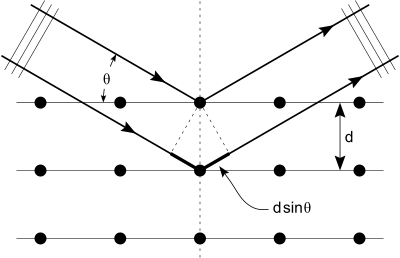
\includegraphics[width=0.45\textwidth]{bragg.png}
     
    \label{fig:bragg}
\end{figure}
% The von Laue approach regards the crystal as composed of identical microscopic objects places at the sites $\Vec{R}$ of a Bravais lattice, each of which can radiate incident radiation in all directions. Sharp peaks are observed only in directions and at wavelengths for which the rays scattered from all lattice points interfere constructively.\\
% Consider now two scatterers separated by a displacement vector $\Vec{d}$. Let an X-ray be incident from very far away along a direction $\hat{n}$ with wavelength $\lambda$ and wave vector $\Vec{k}=2\pi\hat{n}/\lambda$. A scattered ray in the direction $\hat{n}'$ with wavelength $\lambda$ and wave vector $\Vec{k}'=2\pi\hat{n}'/\lambda$. The path difference between the two rays is:
% \[
% \Vec{d}\cdot(\hat{n}-\hat{n}')=d\cos\theta+d\cos\theta'
% \]
% The condition for constructive interference is:
% \[
% \Vec{d}\cdot(\hat{n}-\hat{n}')=m\lambda\Rightarrow\Vec{d}\cdot(\Vec{k}-\Vec{k}')=2\pi m
% \]
% for integer values of $m$. Considering now an array of scatterers at the sites of a Bravais lattice, the condition that all scattered rays interfere constructively is that the condition above holds true for all values of $\Vec{d}$ that are Bravais lattice vectors:
% \[
% \Vec{R}\cdot(\Vec{k}-\Vec{k}')=2\pi m\Rightarrowe^{i(\Vec{k}'-\Vec{k}\cdot\Vec{R})}=1
% \]
% for all Bravais lattice vectors $\Vec{R}$ and integer values of $m$. Comparing this with the definition of reciprocal lattice, it is possible to conclude that the Laue condition states that \textit{constructive interference will occur provided that the change in wave vector $\Vec{k}'-\Vec{k}$ is a vector of the reciprocal lattice.}\\
% This discussion is based on the condition that rays scattered from each primitive cell should interfere constructively. If the crystal structure is that of a monoatomic lattice with an $n-$atom basis, the contents of each primitive cell can be further analysed into a set of identical scatterers at position $\Vec{d_1},\cdots,\Vec{d_n}$ within the cell. If the Bragg peak is associated with a change in wave vector, then the phase difference between the rays scattered at $\Vec{d_i}$ and $\Vec{d_j}$ will be $\Vec{K}\cdot(\Vec{d_i}-\Vec{d_j})$ and the amplitude of the two rays will differ by a factor $e^{i\Vec{K}\cdot(\Vec{d_i}-\Vec{d_j})}$. The amplitudes of the rays scattered at $\Vec{d_1},\cdots,\Vec{d_n}$ are in the ratio $e^{i\Vec{K}\cdot\Vec{d_1}},\cdots,e^{i\Vec{K}\cdot\Vec{d_n}}$. The net ray scattered by the entire primitive cell is the sum of the individual rays, with an amplitude containing the factor:
% \[
% S_{\Vec{K}}=\sum_{j=1}^ne^{i\Vec{K}\cdot\Vec{d_j}}
% \]
% This is known as \textbf{geometrical structure factor}. The intensity in the Bragg peak, proportional to the absolute value of the amplitude, will contain a factor $|S_{\Vec{K}}|^2$.\\
% If the ions in the basis are not identical, the structure factor assumes the form:
% \[
% S_{\Vec{K}}=\sum_{j=1}^nf_j(\Vec{K})e^{i\Vec{K}\cdot\Vec{d_j}}
% \]
% where $f_j$ is known as the \textbf{atomic form factor} and it is entirely determined by the internal structure of the ion that occupies position $\Vec{d_j}$ in the basis. Identical ions have identical form factors, so in the monoatomic case this reduces back to the geometrical structure factor multiplied by the common value of the form factors.
\newpage
\section{Lattice Dynamics of Crystals}
\subsection{The Born-Oppenheimer Approximation}
In a system of many particles interacting via electromagnetic forces, the general problem is to solve the Schr\"odinger equation:
\[
H\Psi=E\Psi
\]
where both the Hamiltonian both the wave function depend on the coordinates of all the particles. The Hamiltonian $H$ can be seen as the sum of different terms:
\[
H=T_e+T_N+V_{NN}+V_{ee}+V_{eN}+C_e^{\text{rel}}
\]
The first one is the kinetic term for the electrons:
\[
T_e=\sum_e\frac{p_e^2}{2m}=-\sum_i\frac{\hbar^2}{2m}\nabla_i^2
\]
where $i$ denotes the coordinates of the electronic positions. The second term regards the kinetic part of the nuclei:
\[
T_N=\sum_N\frac{p_N^2}{2M}=-\sum_I\frac{\hbar^2}{2M}\nabla^2_I
\]
where $I$ denotes the coordinates of the nuclear positions. Then there are the potential terms:
\[
\left\{
\begin{aligned}
&\text{Nuclei interaction:} &&V_{NN}=\frac{1}{2}\sum_{I\neq J}\frac{Z_IZ_Je^2}{4\pi\varepsilon_0|\Vec{R_I}-\Vec{R_J}|}\\
&\text{Electrons interaction:} &&V_{ee}=\frac{1}{2}\sum_{i\neq j}\frac{e^2}{4\pi\varepsilon_0|\Vec{r_i}-\Vec{r_j}|}\\
&\text{Electron-nucleus interaction:} &&V_{eN}=-\sum_{i,J}\frac{Z_Je^2}{4\pi\varepsilon_0|\Vec{r_i}-\Vec{R_J}|}\\
\end{aligned}
\right.
\]
The last term $C_e^{\text{rel}}$ accounts for relativistic corrections on electrons. The Schr\"odinger equation can be simplified by decomposing the wave function in a product of simpler functions:
\[
\Psi_{nv}(\Vec{r},\Vec{R})=F_{n,v}(\Vec{R})\psi_n(\Vec{r},\Vec{R})
\]
$\Vec{r}$ denotes the electronic coordinates while $\Vec{R}$ the nuclear ones. This approximation is due to the enormous difference in speed between nuclei and electrons. For electrons, the speed can be computed by using the virial theorem:
\[
\frac{m_ev^2}{2}\sim\frac{Ze^2}{4\pi\varepsilon_0a_0}\Rightarrow v\sim\sqrt{\frac{Ze^2}{4\pi\varepsilon_0m_e{\color{red}{a_0}}}}=\sqrt{\frac{Ze^2}{4\pi\varepsilon_0m_e}{\color{red}{\frac{Zm_ec\alpha}{\hbar}}}}=Z\alpha c
\]
To estimate the velocity of nuclei, we note that when we try to \textit{pull away} the electron cloud, the nuclei respond elastically. Under the assumption that for the elastic constants $K_e\sim K_N$, we then have:
\[
m_e\omega_e^2\sim M\omega_N^2\xleftrightarrow[]{}\omega_N\sim\sqrt{\frac{m_e}{M}}\omega_e\Rightarrow E_N\sim\sqrt{\frac{m_e}{M}}E_e\Rightarrow v_N\sim\left(\frac{m_e}{M}\right)^{3/4}v_e\sim3\cdot10^{-10}v_e
\]
All in all, this assumption corresponds to the decoupling of electronic and nuclear motion.\\
It is now possible to use this result in the Schr\"odinger equation and see what are the contributions coming from the various terms. The electronic kinetic term gives us:
\[
T_e\Psi_{nv}(\Vec{r},\Vec{R})=-\frac{\hbar^2}{2m}\nabla_r^2\Psi_{nv}(\Vec{r},\Vec{R})=-\frac{\hbar^2}{2m}F_{n,v}(\Vec{R})\nabla_r^2\psi_n(\Vec{r},\Vec{R})
\]
For the nuclear kinetic term instead one obtains:
\begin{align*}
T_N\Psi_{nv}(\Vec{r},\Vec{R})&=-\frac{\hbar^2}{2M}\nabla_R^2\Psi_{nv}(\Vec{r},\Vec{R})\\
&=-\frac{\hbar^2}{2M}\left[\psi_n(\Vec{R},\Vec{r})\nabla_R^2F_{n,v}(\Vec{R})+\cancel{2\nabla_RF_{n,v}(\Vec{R})\nabla_R\psi_n(\Vec{r},\Vec{R})}+\cancel{F_{n,v}(\Vec{R})\nabla_R^2\psi_n(\Vec{r},\Vec{R})}\right]
\end{align*}
The last two terms are neglected because they give a contribution much smaller than the first one, since the electronic wavefunction has a very soft dependence on the variation of the distance between nuclei compared to the dependence of the wavefunction of the nuclei.\\
The Schr\"odinger equation now becomes:
\begin{align*}
&-\frac{\hbar^2}{2m}F_{n,v}(\Vec{R})\nabla_r^2\psi_n(\Vec{r},\Vec{R})-\frac{\hbar^2}{2M}\psi_n(\Vec{R},\Vec{r})\nabla_R^2F_{n,v}(\Vec{R})+\\
&+(V_{ee}+V_{NN}+V_{eN}+C_e^{\text{rel}})F_{n,v}(\Vec{R})\psi_n(\Vec{r},\Vec{R})=EF_{n,v}(\Vec{R})\psi_n(\Vec{r},\Vec{R})
\end{align*}
Dividing everything by $F_{n,v}(\Vec{R})\psi_n(\Vec{r},\Vec{R})$ this gets simplified in:
\[
\underbrace{-\frac{\hbar^2}{2m}\frac{\nabla_r^2\psi_n(\Vec{r},\Vec{R})}{\psi_n(\Vec{r},\Vec{R})}+V_{ee}+V_{eN}+C_e^{\text{rel}}}_{=E_n(\Vec{R})}-\frac{\hbar^2}{2M}\frac{\nabla_R^2F_{n,v}(\Vec{R})}{F_{n,v}(\Vec{R})}+V_{NN}=E
\]
There is a situation of the type $f(x,y)+g(y)=$constant, hence it follows that $f(x,y)=f(y)$. In our case, it means that the first four terms must be independent on $\Vec{r}$ and form a function of $\Vec{R}$ only, denoted with $E_n(\Vec{R})$. We then have:
\[
-\frac{\hbar^2}{2M}\frac{\nabla_R^2F_{n,v}(\Vec{R})}{F_{n,v}(\Vec{R})}+V_{NN}+E_n(\Vec{R})=E
\]
The fundamental state will be given by the minimal energy configuration, i.e. the one corresponding to the minimum of the potential: $V_0:=V_{NN}+E_0(\Vec{R})$.
\subsection{Dynamical Matrix of a Linear Chain}
Consider now a 1D chain of lattice constant $a$ formed by a large number $N$ of atoms of mass $M$. Denote with $u_n$ the longitudinal displacement of the $n$-th atom from the equilibrium position $t_n=na$. Fix the nuclei in the positions $R_n=na+u_n$ and indicate with $E_0(\{u_n\})$ the total ground state energy of the electron-nuclear system. In the study of small oscillations, it is convenient to expand the energy in powers of the displacement $u_n$:
\[
E_0(\{u_n\})=E_0(0)+\frac{1}{2}\sum_{nn'}\underbrace{\frac{\partial^2E_0}{\partial u_n\partial u_{n'}}\Bigr|_{\substack{u_n=u_{n'}=0}}}_{:=D_{nn'}}u_nu_{n'}+\cdots
\]
Truncating the expansion to quadratic terms is called \textbf{harmonic approximation}, the quantity denoted above with $D_{nn'}$ goes under the name of \textbf{interatomic force constants} and the matrix $D$ formed with these $D_{nn'}$ is the \textbf{dynamical matrix}. The force constants $D_{nn'}$ represents the proportionality coefficients connecting the forces acting on the nuclei with the displacements:
\[
F_n=-\frac{\partial E_0}{\partial u_n}=-\sum_{n'}D_{nn'}u_{n'}
\]
From the definition, it is possible to obtain some immediate properties of the matrix $D$.
\begin{mybox}
Dynamical matrix properties
\hrule
\begin{enumerate}\renewcommand{\labelenumi}{\arabic{enumi})}
    \item Real and symmetric: $D_{nn'}=D_{n'n}$
    \item The translational symmetry of the lattice requires that:
    \[
    D_{nn'}=D_{mm'} \quad \text{if}\;\; t_n-t_{n'}=t_m-t_{m'}
    \]
    \item Sum rule: $\sum_{n'}D_{nn'}=0 \quad \forall n$
\end{enumerate}
The latter is a consequence of the fact that the forces vanish when all nuclear displacements are zero or when they are all equal
\end{mybox}
\subsubsection{Monoatomic Chain}
Consider now the classical equation of motion for the $n$-th nucleus of mass $M$ in the position $R_n=na+u_n$ under the force $F_n$:
\[
M\Ddot{u}_n=-\sum_{n'=1}^ND_{nn'}u_{n'} \quad n=1,2,\cdots,N
\]
This set of differential equations can be solved by looking for periodic solutions of the form $u_n(t)=Ae^{i(qna-\omega t)}$ where the amplitudes $A$ of the displacements are the same for all sites and the phases are controlled by the Bloch theorem. Substituting this type of solution in the equation above gives us:
\[
-M\omega^2A=-\sum_{n'=1}^ND_{nn'}e^{-iq(na-n'a')}A\Rightarrow M\omega^2(q)=D(q) \quad D(q)=\sum_{n'=1}^ND_{nn'}e^{-iq(na-n'a')}
\]
The Fourier transform $D(q)$ of the force constant matrix elements does not depend on the specific value $n$ because of translational symmetry.\\
We now apply this analysis to the case of a linear chain of atoms with \textbf{nearest neighbour interactions} only. This condition means that the only force constants different from zero are $D_{nn}, D_{nn+1}$ and $D_{n-1n}$ and from propertty 3) of the force constants there is a unique independent parameter, $C$:
\[
D_{nn}=2C \qquad D_{nn+1}=D_{n-1n}=-C
\]
The classical equations of motion now become:
\[
M\Ddot{u}_n=-C(2u_n-u_{n-1}-u_{n+1})
\]
Performing the same substitution as before with $u_n(t)=Ae^{i(qna-\omega t)}$ one obtains:
\[
-M\omega^2=-C(2-e^{iqa}-e^{-iqa})=-4C\sin^2(qa/2)\Rightarrow\omega(q)=\sqrt{\frac{4C}{M}}|\sin(qa/2)|
\]
\begin{figure}[h]
    \centering
    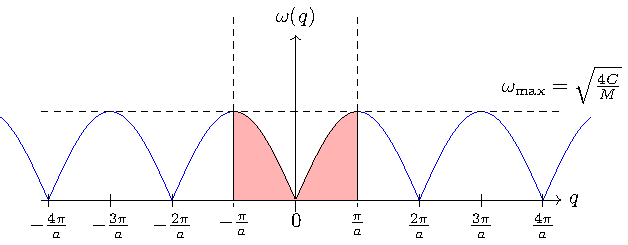
\includegraphics{omega(q).pdf}
    \label{fig:omega(q)}
\end{figure}\\
\noindent 
Notice that the spectrum of vibrational frequencies extends from zero to a cutoff frequency of $\omega_{\max}=\sqrt{4C/M}$ and the whole meaningful physical information is contained inside the \nth{1} Brillouin zone, highlighted in red.\\
In the long wavelength limit, i.e. $qa\ll1$, the dispersion relation takes the form:
\[
\omega(q)\simeq\sqrt{\frac{C}{M}}a|q|=v_s|q| 
\]
The proportionality coefficient $v_s$ between phonon frequency and phonon wave number represents the velocity of the sound in the medium.\\
The ratio between the amplitudes of two nearest neighbours is given by:
\[
\frac{u_{n+1}}{u_n}=\frac{Ae^{i(qna+qa-\omega t)}}{Ae^{i(qna-\omega t)}}=e^{iqa}
\]
Suppose now to have $|q|>\pi/a$ outside of the \nth{1} Brillouin zone, so $q=q'+2\pi n/a$ with $q'\in[-\pi/a,+\pi/a]$. If we take now the ratio we get:
\[
\frac{u_{n+1}}{u_n}=e^{iq'a}e^{2\pi in}
\]
We get the same type of results for vectors outside of the \nth{1} Brillouin zone. It is also possible to compute the group velocity, defined as follows:
\[
v_g=\frac{d\omega}{dq}=\sqrt{\frac{a^2C}{M}}\cos(qa/2)
\]
which vanishes for $q=\pm\pi/a$, on the boundaries of the \nth{1} Brillouin zone. For this value of $q$, the amplitude for $u_n$ takes the form:
\[
u_n=Ae^{i(qna-\omega t)}=A(-1)^ne^{-i\omega t}
\]
This is a stationary wave which can be obtained as a combination of progressive and regressive wave:
\[
A[\sin(kx-\omega t)+\sin(kx+\omega t)]=2A\sin(kx)\cos(\omega t)
\]
How many values of $q$ are in the \nth{1} Brillouin zone?
\[
\#q=\frac{\text{length of $q$}}{\Delta q}=\frac{2\pi/a}{\Delta q}
\]
It seems like the question has been moved to \textit{what is the value of $\Delta q$?} We impose periodic conditions: the atom labeled with $n$ is equivalent to the one labeled with $n+N$, where $N$ is the number of atoms. Using this assumption, we get:
\[
u_n=Ae^{iqna}e^{-i\omega t}=u_{n+N}=Ae^{iq(n+N)a}e^{-i\omega t}\Rightarrow e^{iqNa}=1
\]
This is telling us that $qNA=2\pi m$, with $m\in\mathbb{Z}$, hence $\Delta q=2\pi/Na$ and therefore $\#q=N$.\\
It is now possible to evaluate the number of of phononic states that can be accommodated in a unit volume. Starting from the definition of density of states $D(\omega)=\frac{dN}{d\omega}\frac{1}{V}$, we first compute $dN$:
\[
dN=\frac{2dq}{\Delta q}=\frac{2dq}{\frac{2\pi}{L}}=\frac{L}{\pi}dq
\]
where the factor $2$ has been included to take into account the contribution of negative and positive interval. The density of states then becomes:
\[
D(\omega)=\frac{L}{\pi L}\frac{dq}{d\omega}=\frac{1}{\pi}\frac{dq}{d\omega}=\frac{1}{\pi v_g}
\]
This argument can be easily generalized to two and three dimensions.
\[
\text{2D:}\quad D(\omega)=\frac{q}{2\pi}\frac{dq}{d\omega} \qquad \text{3D:}\quad D(\omega)=\frac{q^2}{2\pi^2}\frac{dq}{d\omega}
\]
\subsubsection{Diatomic Chain}
Consider now the dynamics of a diatomic linear chain of lattice constant $a_0$ with two atoms of mass $M_1$ and $M_2$ in the unit cell. In the equilibrium configuration, assume that the atoms of mass $M_1$ occupy the position $R_n^{(1)}=na_0$ while the atoms of mass $M_2$ occupy $R_n^{(2)}=(n+1/2)a_0$. $u_n$ indicates the displacements of the atoms of mass $M_1$ and $v_n$ the displacements of the atoms of mass $M_2$. Again, we work in the assumption that only nearest neighbours interact with two different elastic constants: $C_1$ if the interaction is between atoms of the same cell and $C_2$ if it is between atoms of adjacent cells.
\begin{figure}[h]
    \centering
    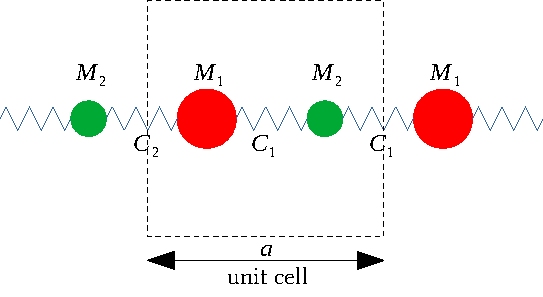
\includegraphics{diatomic_chain.pdf}
     
    \label{fig:diatomic_chain}
\end{figure}\\
\noindent
The equations of motion are:
\[
\left\{
\begin{aligned}
&M_1\Ddot{u}_n=-C_1(u_n-v_n)-C_2(u_n-v_{n-1})\\
&M_2\Ddot{v}_n=-C_1(v_n-u_n)-C_2(v_n-u_{n+1})
\end{aligned}
\right.
\]
The periodic solutions for $u_n$ and $v_n$ now takes the form:
\[
u_n(t)=A_ue^{i(qna-\omega t)} \qquad v_n(t)=A_ve^{i(qna-\omega t)}
\]
Substituting them in the equations above gives us:
\[
\left\{
\begin{aligned}
&-M_1\omega^2A_u=-C_1(A_u-A_v)-C_2(A_u-A_ve^{-iqa})\\
&-M_2\omega^2A_v=-C_1(A_v-A_u)-C_2(A_v-A_ue^{iqa})
\end{aligned}
\right.
\to
\left\{
\begin{aligned}
&A_u(-M_1\omega^2+C_1+C_2)=A_v(C_1+C_2e^{-iqa})\\
&A_v(-M_2\omega^2+C_1+C_2)=A_u(C_1+C_2e^{iqa})
\end{aligned}
\right.
\]
This system of equations have a non-trivial solution if the determinant of the coefficient matrix of $A_u$ and $A_v$ is zero.
\[
\det\left(\begin{array}{cc}
    C_1+C_2-M_1\omega^2 & C_1+C_2e^{iqa} \\
    C_1+C_2e^{-iqa} & C_1+C_2-M_2\omega^2
\end{array}\right)=0
\]
Imposing the determinant to be equal to 0 gives us a second degree equation in $\omega^2$ whose solutions are:
\[
\omega^2=\frac{(C_1+C_2)(M_1+M_2)}{2M_1M_2}\pm\sqrt{\frac{(C_1+C_2)^2(M_1+M_2)^2}{4(M_1M_2)^2}-\frac{4C_1C_2\sin^2(qa/2)}{M_1M_2}}
\]
The main difference with the monoatomic case is that here for each $q$ there are two possible values of $\omega$ instead of one.
\begin{figure}[h]
    \centering
    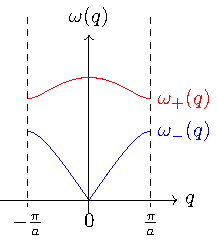
\includegraphics{omega+-.pdf}
    \label{fig:omega+-}
\end{figure}\\
\noindent
The $(+)$ solution corresponds to the \textbf{optical branch} while the $(-)$ solution is the \textbf{acoustic branch}. In the case $C_1=C_2=C$ we get:
\[
\omega^2=C\left(\frac{1}{M_1}+\frac{1}{M_2}\right)\pm C\sqrt{\left(\frac{1}{M_1}+\frac{1}{M_2}\right)^2-\frac{4\sin^2(qa/2)}{M_1M_2}}
\]
A further simplification is given by the case in which $C_1=C_2=C$ and $M_1=M_2=M$:
\[
\omega_+=\sqrt{\frac{4C}{M}}\cos(qa/4) \qquad \omega_-=\sqrt{\frac{4C}{M}}\sin(qa/4)
\]
The amplitudes $A_u$ and $A_v$ satisfies the relation:
\[
\frac{A_u}{A_v}=\frac{C_1+C_2e^{iqa}}{C_1+C_2-M_1\omega^2}=\frac{C_1+C_2-M_2\omega^2}{C_1+C_2e^{iqa}}
\]
Consider now the case in which $M_1=M_2=M$ but $C_1\neq C_2$ and work in the long wavelength limit, i.e. $qa\ll1$.
\[
\omega^2=\frac{C_1+C_2}{M}\pm\frac{1}{M}\sqrt{C_1^2+C_2^2+2C_1C_2\cos(qa)}\simeq\frac{C_1+C_2}{M}\pm\frac{1}{M}\sqrt{C_1^2+C_2^2+2C_1C_2\left(1-\frac{q^2a^2}{2}+\mathcal{O}((qa)^4)\right)}
\]
The $(+)$ and $(-)$ solutions, i.e. respectively the optical and acoustic branch, now become:
\[
\left\{
\begin{aligned}
&\text{Optical branch}: &&\omega\simeq\sqrt{\frac{2(C_1+C_2)}{M}}+\mathcal{O}((qa)^2) &&&\frac{A_u}{A_v}=-1 &&&v_g=0\\
&\text{Acoustic branch}: &&\omega\simeq\sqrt{\frac{C_1C_2}{2M(C_1+C_2)}}qa &&&\frac{A_u}{A_v}=+1 &&&v_g=\sqrt{\frac{C_1C_2}{2M(C_1+C_2)}}a
\end{aligned}
\right.
\]
In the acoustic branch in the long wavelength limit, the atoms vibrate in phase and with the same amplitude and the frequency $\omega$ is proportional to the wave number $q$. In the optical branch, $A_u$ and $A_v$ have opposite signs and the group velocity vanishes: the two atoms in the unit cell move in opposite directions while the \textit{center of mass} of the unit cell remains fixed.
\subsection{Linear Chain Hamiltonian: \RN{1} Quantization}
So far, we have considered the classical dynamics of a linear chain. Now we move to the quantum mechanical counterpart of the same problem. Working in the harmonic approximation and considering only nearest neighbour interactions, the Hamiltonian of the linear chain becomes:
\begin{equation}
\label{H}
H=\sum_n\frac{p_n^2}{2M}+\frac{1}{2}C\sum_n(2u_n^2-u_nu_{n+1}-u_nu_{n-1})
\end{equation}
where $u_n$ and $p_n$ are the coordinate and the conjugate momentum of the nucleus respectively at the $n$-th site, which satisfies the usual commutation relations.
\[
[u_n,p_{n'}]=i\hbar\delta_{nn'} \qquad [u_n,u_{n'}]=[p_n,p_{n'}]=0
\]
However, instead of working with them it is more convenient to perform a canonical transformation, with the final aim to put the Hamiltonian in the diagonal form.
\[
p_q=\frac{1}{\sqrt{N}}\sum_{t_n}p_ne^{+iqt_n} \qquad u_q=\frac{1}{\sqrt{N}}\sum_{t_n}u_ne^{-iqt_n}
\]
where $t_n=na$. The inverse transformations are given by:
\[
p_n=\frac{1}{\sqrt{N}}\sum_qp_qe^{-iqt_n} \qquad u_n=\frac{1}{\sqrt{N}}\sum_qu_qe^{+iqt_n}
\]
It is easy to see that these transformations are canonical, i.e. the commutation rules are preserved.
\[
[u_q,p_{q'}]=i\hbar\delta_{qq'} \qquad [u_q,u_{q'}]=[p_q,p_{q'}]=0
\]
It is now possible to express the original Hamiltonian in terms of the new displacements and conjugated momenta.
\[
\left\{
\begin{aligned}
&\sum_np_n^2=\sum_n\frac{1}{N}\sum_q\sum_{q'}p_qp_{q'}e^{-i(q+q')t_n}=\sum_qp_qp_{-q}\\
&\sum_nu_n^2=\sum_n\frac{1}{N}\sum_q\sum_{q'}u_qu_{q'}e^{i(q+q')t_n}=\sum_qu_qu_{-q}\\
&\sum_nu_nu_{n+1}=\sum_n\frac{1}{N}\sum_q\sum_{q'}u_qu_{q'}e^{i(q+q')t_n+iq'a}=\sum_qu_qu_{-q}e^{-iqa}\\
&\sum_nu_nu_{n-1}=\sum_n\frac{1}{N}\sum_q\sum_{q'}u_qu_{q'}e^{i(q+q')t_n-iq'a}=\sum_qu_qu_{-q}e^{+iqa}
\end{aligned}
\right.
\]
In every last passage of the relations above, we used the fact that $\frac{1}{N}\sum_ne^{i(q+q')t_n}=\delta(q-q')$.\\
The Hamiltonian of \hyperref[H]{Equation (\ref{H})} can now be written as:
\begin{equation}
\label{H1}
H=\sum_q\frac{p_qp_{-q}}{2M}+\frac{1}{2}C\sum_qu_qu_{-q}(2-e^{-iqa}+e^{+iqa})=\sum_q\left[\frac{p_qp_{-q}}{2M}+\frac{1}{2}M\omega^2(q)u_qu_{-q}\right]
\end{equation}
where $\omega^2(q)$ is given by the following:
\[
\omega^2(q)=\frac{C}{M}(2-e^{-iqa}+e^{+iqa})=\frac{4C}{M}\sin^2(qa/2)
\]
This shows that the linear chain of $N$ coupled harmonic oscillators is equivalent to $N$ uncoupled normal modes.\\
It is useful to define another canonical transformation to creation and destruction operators, so we define:
\[
a_q=\sqrt{\frac{m\omega(q)}{2\hbar}}u_q+i\sqrt{\frac{1}{2M\hbar\omega(q)}}p_{-q} \qquad a_q^\dagger=\sqrt{\frac{m\omega(q)}{2\hbar}}u_{-q}-i\sqrt{\frac{1}{2M\hbar\omega(q)}}p_q
\]
The commutation rules are preserved:
\[
[a_q,a_{q'}^\dagger]=\delta_{qq'} \quad [a_q,a_{q'}]=[a_q^\dagger,a_{q'}^\dagger]=0
\]
The displacements and the conjugated momenta gets now written in the form:
\[
\left\{
\begin{aligned}
&u_n=\frac{1}{\sqrt{N}}\sum_q\overbrace{\sqrt{\frac{\hbar}{2M\omega(q)}}(a_q+a_{-q}^\dagger)}^{u_q}e^{+iqt_n}\\
&p_n=\frac{1}{\sqrt{N}}\sum_q\underbrace{(-i)\sqrt{\frac{M\hbar\omega(q)}{2}}(a_{-q}-a_q^\dagger)}_{p_q}e^{-iqt_n}
\end{aligned}
\right.
\]
The Hamiltonian of \hyperref[H1]{Equation (\ref{H1})} can be expressed in second quantization form:
\[
H=\sum_q\hbar\omega(q)\left(a_q^\dagger a_q+\frac{1}{2}\right)
\]
which can be seen as the sum of the Hamiltonians of $N$ independent linear harmonic oscillators of frequency $\omega(q)$.
\subsection{Lattice Dynamics in 3D}
The lattice dynamics discussed before was the one of a 1D crystal, now we address the general problem of a 3D crystal. Consider a general 3D crystal with $N$ unit cells, translation vectors $\Vec{t_n}$ and a basis of atoms in the positions $\Vec{d}_1,\Vec{d}_2,\cdots,\Vec{d}_n$. The generic position vector is given by $\Vec{t}_n+\Vec{d}_\nu+\Vec{u}_{n\nu}$ and the energy of the electronic-nuclear system is denoted by $E_0(\{\Vec{u}_{n\nu}\})$. The expansion up to second order gives us:
\[
E_0(\{\Vec{u}_{n\nu}\})=E_0(0)+\frac{1}{2}\sum_{n\nu\alpha,n'\nu'\alpha'}D_{n\nu\alpha,n'\nu'\alpha'}u_{n\nu\alpha}u_{n'\nu'\alpha'}
\]
where $\alpha,\alpha'=x,y,z$; $\nu,\nu'=1,\cdots,\nu_b$ where $\nu_b$ is the number of atoms forming the basis of the unit cell and $n=1,\cdots,N$. Explicitly, the interatomic force constants are defined as:
\[
D_{n\nu\alpha,n'\nu'\alpha'}=\frac{\partial^2E_0}{\partial u_{n\nu\alpha}\partial u_{n'\nu'\alpha'}}\Bigr|_{\substack{0}}
\]
The matrix $D$ is called the \textbf{dynamical matrix of the crystal in real space} and it has some properties:
\begin{mybox}
3D dynamical matrix properties
\hrule
\begin{enumerate}\renewcommand{\labelenumi}{\arabic{enumi})}
    \item It is real and symmetric: $D_{n\nu\alpha,n'\nu'\alpha'}=D_{n'\nu'\alpha',n\nu\alpha}$
    \item Translational symmetry implies: 
    \[
    D_{n\nu\alpha,n'\nu'\alpha'}=D_{m\nu\alpha,m'\nu'\alpha'} \quad\text{if}\; \Vec{t}_n-\Vec{t}_{n'}=\Vec{t}_m-\Vec{t}_{m'}
    \]
    \item Sum rule: $\sum_{n'\nu'}=D_{n\nu\alpha,n'\nu'\alpha'}=0$
\end{enumerate}
\end{mybox}
\noindent
In the harmonic approximation, the classical equations of motion read:
\[
M_\nu\Ddot{u}_{n\nu\alpha}=-\sum_{n'\nu'\alpha'}D_{n\nu\alpha,n'\nu'\alpha'}u_{n'\nu'\alpha'}
\]
Again, this set of differential equations is solved by looking for solutions in the form:
\[
\Vec{u}_{n\nu}(t)=\Vec{A}_\nu(\Vec{q},\omega)e^{i(\Vec{q}\cdot\Vec{t}_n-\omega t)}
\]
Replacing this solution in the equation above gives us:
\[
-M_\nu\omega^2A_{\nu\alpha}=-\sum_{n'\nu'\alpha'}D_{n\nu\alpha,n'\nu'\alpha'}A_{\nu'\alpha'}e^{-i\Vec{q}(\Vec{t}_n-\Vec{t}_{n'})}
\]
Non-trivial solutions are obtained by solving the following:
\[
\det[D_{\nu\alpha,\nu'\alpha'}(\Vec{q})-M_\nu\omega^2\delta_{\alpha\alpha'}\delta_{\nu\nu'}]=0 \quad \text{where}\;\; D_{\nu\alpha,\nu'\alpha'}(\Vec{q})=\sum_{n'}D_{n\nu\alpha,n'\nu'\alpha'}e^{-i\Vec{q}\cdot(\Vec{t}_n-\Vec{t}_{n'})}
\]
The matrix $D(\Vec{q})$ has dimension $3\nu_b$, the secular equation produces $3\nu_b$ eigenvalues, called phonons or normal modes. At every vector $\Vec{q}$ there are $3\nu_b$ normal modes, giving rise to $3\nu_b$ phonon branches as $\Vec{q}$ varies inside the \nth{1} Brillouin zone. Let $\omega(\Vec{q},p)$ be the frequency of the $p$-th normal mode of wave vector $\Vec{q}$ and $\Vec{A}_\nu(\Vec{q},p)$ the corresponding polarization vectors. A mode $\omega(\Vec{q},p)$ is called \textbf{longitudinal} in case the polarization vectors $\Vec{A}_\nu(\Vec{q},p)$ are parallel to $\Vec{q}$, while it is called \textbf{transverse} if they are perpendicular to it.
\newpage
\section{Thermal Properties}
We have seen that the energy of the states of the crystal is given by the eigenvalues of the Hamiltonian in \hyperref[H1]{Equation (\ref{H1})} from which it follows using the equipartition theorem that the internal energy per unit of volume is:
\[
u=\frac{1}{V}\left(\frac{1}{2}k_BT+\frac{1}{2}k_BT\right)3N=3nk_BT \quad \text{where}\;\;n=\frac{N}{V}
\]
From this, it is possible to obtain the specific heat $c_v$ by simply deriving with respect to the temperature:
\[
c_v=\frac{\partial u}{\partial T}=3nk_B
\]
which is not what it is observed experimentally. This is a purely classical result in which the discretization of the energy levels is neglected but at low temperatures the quantization of the amplitude of the lattice vibrations become important. We explicitly compute $u$ given by:
\[
u=\frac{1}{V}\frac{\sum_iE_ie^{-\beta E_i}}{\sum_ie^{-\beta E_i}}=-\frac{\partial f}{\partial\beta} \quad \text{where}\;\;f=\frac{1}{V}\ln{\sum_ie^{-\beta E_i}}
\]
As usual, $\beta=1/k_BT$, $E_i$ is the energy of the $i$-th state of the crystal and the sum is extended over all possible states. The contribution to the total energy of a particular mode with angular frequency $\omega_s(\Vec{q})$ can have only a discrete set of values:
\[
E_{n_{\Vec{q}s}}=\hbar\omega_s(\Vec{q})\left(n_{\Vec{q}s}+\frac{1}{2}\right)
\]
where $n_{\Vec{q}s}$ is the excitation number of the mode. The term $\sum_ie^{-\beta E_i}$ can be calculated:
\begin{align*}
\sum_ie^{-\beta E_i}&=\sum_{\{n_{\Vec{q}s}\}}e^{-\beta\sum_{\{n_{\Vec{q}s}\}}\hbar\omega_s(\Vec{q})\left(n_{\Vec{q}s}+\frac{1}{2}\right)}=\sum_{\{n_{\Vec{q}s}\}}\prod_{\Vec{q}s}e^{-\beta\hbar\omega_s(\Vec{q})\left(n_{\Vec{q}s}+\frac{1}{2}\right)}\\
&=\prod_{\Vec{q}s}\sum_{n_{\Vec{q}s}}e^{-\beta\hbar\omega_s(\Vec{q})\left(n_{\Vec{q}s}+\frac{1}{2}\right)}=\prod_{\Vec{q}s}e^{-\beta\hbar\omega_s(\Vec{q})/2}\sum_{n_{\Vec{q}s}}e^{-\beta\hbar\omega_s(\Vec{q})n_{\Vec{q}s}}\\
&=\prod_{\Vec{q}s}\frac{e^{-\beta\hbar\omega_s(\Vec{q})/2}}{1-e^{-\beta\hbar\omega_s(\Vec{q})}}
\end{align*}
Here we are treating the phonons as bosons. At the end of the day one gets:
\[
f=\frac{1}{V}\ln{\prod_{\Vec{q}s}\frac{e^{-\beta\hbar\omega_s(\Vec{q})/2}}{1-e^{-\beta\hbar\omega_s(\Vec{q})}}}=\frac{1}{V}\sum_{\Vec{q}s}\ln{\frac{e^{-\beta\hbar\omega_s(\Vec{q})/2}}{1-e^{-\beta\hbar\omega_s(\Vec{q})}}}
\]
By differentiating $f$ with respect to $\beta$, the internal energy density $u$ assumes the form:
\[
u=-\frac{\partial f}{\partial\beta}=\frac{1}{V}\sum_{\Vec{q}s}\hbar\omega_s(\Vec{q})\left(n_s(\Vec{q})+\frac{1}{2}\right) \quad \text{where}\;\; n_s(\Vec{q})=\frac{1}{e^{\beta\hbar\omega_s(\Vec{q})}-1}
\]
In the quantum theory of the harmonic solid, the specific heat is no longer constant but given by:
\[
c_v=\frac{\partial u}{\partial T}=\frac{1}{V}\sum_{\Vec{q}s}\frac{\partial}{\partial T}\frac{\hbar\omega_s(\Vec{q})}{e^{\beta\hbar\omega_s(\Vec{q})}-1}
\]
In the limit $\beta\hbar\omega\ll1$, i.e. high-temperature limit, the specific heat can be approximated as:
\[
c_v\simeq\frac{1}{V}\sum_{\Vec{q}s}\frac{\partial}{\partial T}\frac{\hbar\omega_s(\Vec{q})}{\beta\hbar\omega_s(\Vec{q})}=\frac{1}{V}\sum_{\Vec{q}s}k_B\frac{\partial T}{\partial T}=\frac{1}{V}3Nk_B=3nk_B
\]
This tells us that the classical result is recovered in the high-temperature limit. On the other hand, moving to the low-temperature regime, i.e. $\beta\hbar\omega\gg1$, we observe that the set of discrete wave vectors which we summed over becomes dense on the scale over which the summand has an appreciable variation. Therefore, the sum is replaced by an integral:
\begin{equation}
\label{general}
c_v=\frac{\partial}{\partial T}\sum_s\int_{\text{\RN{1}BZ}}\frac{d\Vec{q}}{(2\pi)^3}\frac{\hbar\omega_s(\Vec{q})}{e^{\beta\hbar\omega_s(\Vec{q})}-1}
\end{equation}
where the integral is taken over the \nth{1} Brillouin zone. At very low temperature, modes with $\hbar\omega_s(\Vec{q})\gg k_BT$ contribute negligibly to the integral, since the integrand will vanish exponentially. This condition will not be satisfied by acoustic modes of sufficiently long wavelength, since $\omega_s(\Vec{q})\to0$ as $\Vec{q}\to0$. These modes will continue to contribute appreciably to $c_v$. With this in mind, we can make some simplifications:
\begin{enumerate}
    \item It is possible to ignore the optical modes in the sum over $s$
    \item We can replace $\omega_s(\Vec{q})$ for the acoustic branches with its long wavelength form $c_s(\hat{\Vec{q}})q$
    \item The integration can be extended over all the $q$-space because the integrand is small unless $\hbar c_s(\hat{\Vec{q}})q$ is of order $k_BT$, which happens in the proximity of $\Vec{q}=\Vec{0}$ at low temperatures
\end{enumerate}
\begin{figure}[h]
    \centering
    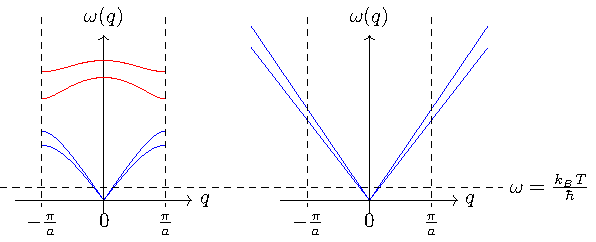
\includegraphics{simplifications.pdf}
    \label{fig:simplifications}
\end{figure}
With these approximations, at very low temperatures the expression for the specific heat gets simplified as:
\[
c_v=\frac{\partial}{\partial T}\sum_s\int\frac{d\Vec{q}}{(2\pi)^3}\frac{\hbar c_s(\hat{\Vec{q}})q}{e^{\beta\hbar c_s(\hat{\Vec{q}})q}-1}
\]
The integral gets evaluated in spherical coordinates, $d\Vec{q}=dqd\Omega q^2$, and by performing a change of variables $\beta\hbar c_s(\hat{\Vec{q}})q=x$.
\[
c_v=\frac{\partial}{\partial T}\sum_s\int\frac{d\Omega}{8\pi^3}\frac{(k_BT)^4}{(\hbar c_s)^3}\int_0^\infty dx\frac{x^3}{e^x-1}
\]
The sum on $s$ gives us the average of the long wavelength phase velocities of the three acoustic modes:
\[
\sum_s\frac{1}{c_s^3}=\frac{1}{c_L^3}+\frac{2}{c_T^3}=\frac{3}{c^3}
\]
For the remaining two pieces, we have:
\[
\int\frac{d\Omega}{8\pi^3}=\frac{4\pi}{8\pi^3}=\frac{1}{2\pi^2} \qquad \int_0^\infty dx\frac{x^3}{e^x-1}=\Gamma(4)\zeta(4)=3!\frac{\pi^4}{90}=\frac{\pi^4}{15}
\]
Putting everything together we finally obtain:
\[
c_v=\frac{\partial}{\partial T}\frac{\pi^2}{10}\frac{(k_BT)^4}{(\hbar c)^3}=\frac{2\pi^2}{5}k_B\left(\frac{k_BT}{\hbar c}\right)^3\sim T^3
\]
which agrees with the experimental results.
\subsection{Debye-Einstein Model}
There is still a considerable temperature range over which neither the high- nor the low-temperature limit work and one has to work with the general form [\hyperref[general]{Equation (\ref{general})}]. Nevertheless, it is common to use an approximate interpolation scheme for this intermediate temperature range.\\
The \textbf{Debye model} replaces all branches of the vibrational spectrum with three branches, each of them characterized by $\omega=cq$. Moreover, the integral over the \nth{1} Brillouin zone is replaced by an integral over a sphere of radius $q_D$ chosen to contain precisely $N$ allowed wave vectors, where $N$ is the number of ions in the crystal. This requires:
\[
\frac{4}{3}\pi q_D^3=\frac{N}{V}(2\pi)^3\Rightarrow n=\frac{q_D^3}{6\pi^2}
\]
As a result of this simplification, \hyperref[general]{Equation (\ref{general})} becomes:
\[
c_v=\frac{\partial}{\partial T}\sum_s\frac{\hbar c_s}{2\pi^2}\int_0^{q_D}dq\frac{q^3}{e^{\beta\hbar c_sq}-1}=\frac{3\hbar c}{2\pi^2}\int_0^{q_D}dq\frac{q^3}{(e^{\beta\hbar cq}-1)^2}e^{\beta\hbar cq}\frac{\hbar cq}{k_BT^2}
\]
The integral is computed by performing a change of variables, defining $x=\hbar cq/k_BT=\beta\hbar cq$ and a Debye temperature $k_B\Theta_D=\hbar cq_D$:
\[
c_v=\frac{3k_B^4T^3}{2\pi^2(\hbar c)^3}\int_0^{x_D}dx\frac{x^4e^x}{(e^x-1)^2}=\frac{3k_B^4T^3q_D^3}{2\pi^2k_B^3\Theta_D^3}\int_0^{x_D}dx\frac{x^4e^x}{(e^x-1)^2}\underset{\mathclap{\tikz \node {$\uparrow$} node [below=1ex] {\footnotesize $q_D^3=6\pi^2n$};}}{=}9nk_B\left(\frac{T}{\Theta_D}\right)^3\int_0^{x_D}dx\frac{x^4e^x}{(e^x-1)^2}
\]
We can check the goodness of this model by looking at the high- and low-temperature limits:
\[
\left\{
\begin{aligned}
&\bullet\underset{(x\to0)}{T\to\infty:}&&c_V\simeq9nk_B\left(\frac{T}{\Theta_D}\right)^3\int_0^{x_D}dx\frac{x^4(1+x+\cdots)}{(1+x+\cdots-1)^2}=9nk_B\left(\frac{T}{\Theta_D}\right)^3\int_0^{x_D}dxx^2\\
& &&{\color{white}{c_V}}=9nk_B\left(\frac{T}{\Theta_D}\right)^3\frac{x_D^3}{3}=3nk_B \quad \checkmark\\
&\bullet\underset{(x\to\infty)}{T\to0:}&&c_V\simeq9nk_B\left(\frac{T}{\Theta_D}\right)^3\int_0^\infty dx\frac{x^4e^x}{(e^x-1)^2}=9nk_B\left(\frac{T}{\Theta_D}\right)^3\frac{4\pi^4}{15}\\
& &&{\color{white}{c_V}}=\frac{12\pi^4}{5}nk_B\left(\frac{T}{\Theta_D}\right)^3\sim T^3 \quad \checkmark
\end{aligned}
\right.
\]
At high temperature, we recover the Dulong-Petit limit, provided that the crystal is monoatomic. This is related to the fact that acoustic cells are blind with respect to the basis.\\
In the Debye model of a crystal with a polyatomic basis, the optical branches of the spectrum are represented by the high $q$ values of the expression $\omega=cq$, while the low $q$ values give the acoustic branch. An alternative scheme is to apply the Debye model only to the three acoustic branches of the spectrum. The optical branches are represented by the \textbf{Einstein model}, which replaces the frequency of each optical branch by a frequency $\omega_E$ that does not depend on $\Vec{q}$. The density $n$ is now the number of primitive cells per unit volume of crystal and the expression for $c_V$ provided by the Debye model accounts only for the contribution of the acoustic branches. For each optical branch, the thermal energy density is given by:
\[
u=\frac{n\hbar\omega_E}{e^{\beta\hbar\omega_E}-1}
\]
This has to be multiplied by the number of optical branches $p$, so that there will be an additional contribution to the specific heat of the form:
\[
c_V^{\text{optical}}=pnk_B\frac{e^{\beta\hbar\omega_E}}{(e^{\beta\hbar\omega_E}-1)^2}\left(\frac{\hbar\omega_E}{k_BT}\right)^2
\left\{
\begin{aligned}
&T\to\infty: &&c_V^{\text{optical}}\simeq pnk_B\\
&T\to0: &&c_V^{\text{optical}}\simeq e^{-\beta\hbar\omega_E}
\end{aligned}
\right.
\]
For very low temperature, the contribution from optical branches is negligible. Summing the contribution of acoustic and optical branches at high temperature gives us:
\[
c_V\sim3nk_B+pnk_B=3nk_B+nk_B[3(s-1)]=3nsk_B
\]
where $s$ is the number of atoms in the basis and in 3D we have that $p=3(s-1)$.\\
For very low temperatures, the Debye model gives correct results, while there are some discrepancies at medium temperatures. Such discrepancies are due to the fact that, as the temperature increases, phonons of higher frequency are created. It is then needed to take into account the real dispersion curves of the crystal and compute for each of them the density of states $D(\omega)$, given by:
\[
D(\omega)d\omega=\frac{V}{(2\pi)^3}\int_\Delta d\Vec{q}
\]
where the integral is extended over a volume $\Delta$ of the $\Vec{q}$ space where the frequency is between $\omega$ and $\omega+d\omega$. Consider now two surfaces, one identified by $\omega(q)=\omega$ and the other by $\omega(q)=\omega+d\omega$ infinitely close. The following relation holds true:
\[
d\omega=\frac{\partial\omega}{\partial q_x}dq_x+\frac{\partial\omega}{\partial q_y}dq_y+\frac{\partial\omega}{\partial q_z}dq_z=\Vec{\nabla}_{\Vec{q}}\omega\cdot d\Vec{q}=|\Vec{\nabla}_{\Vec{q}}\omega|dq_\perp
\]
because $\Vec{\nabla}_{\Vec{q}}\omega$ is perpendicular to the surface $\omega(q)=\omega$. We can exploit this fact by writing: 
\[
d\Vec{q}=dS_\omega\cdot dq_\perp=\frac{dS_\omega}{|\Vec{\nabla}_{\Vec{q}}\omega|}d\omega
\]
which gives a much more convenient expression for the density of states:
\[
D(\omega)d\omega=\frac{V}{(2\pi)^3}\left[\int_S\frac{dS_\omega}{|\Vec{v}_g|}\right] \quad \text{equivalently} \quad D(\omega)=\frac{V}{(2\pi)^3}\int d\Vec{q}\delta[\omega(\Vec{q})-\omega]
\]
Another way to compute $D(\omega)$ in 3D is to write:
\[
D(\omega)=\frac{dN}{d\omega}=\frac{1}{d\omega}\frac{d^3q}{\frac{(2\pi)^3}{V}}=\frac{q^2V}{2\pi^2}\frac{dq}{d\omega}\overset{\mathclap{\tikz \node {$\downarrow$} node [above=1ex] {\footnotesize $\omega=cq$};}}{=}\frac{\omega^2V}{2\pi^2c^3}
\]
Similarly, in 2D and 1D one has:
\[
\left\{
\begin{aligned}
&\text{2D:} &&D(\omega)=\frac{dN}{d\omega}=\frac{1}{d\omega}\frac{d^2q}{\frac{(2\pi)^2}{S}}=\frac{qS}{2\pi}\frac{dq}{d\omega}=\frac{\omega S}{2\pi c^2}\\
&\text{1D:} &&D(\omega)=\frac{dN}{d\omega}=\frac{1}{d\omega}\frac{2dq}{\frac{(2\pi)}{L}}=\frac{qL}{\pi}\frac{dq}{d\omega}=\frac{L}{\pi c}
\end{aligned}
\right.
\]
Another source of specific heat is represented, for metals, by the electrons. In a metal there is an underlying lattice and a \textit{sea} of electrons with dispersion curve given by:
\[
E(\Vec{k})\simeq\frac{\hbar^2k^2}{2m_e}
\]
To determine the energy density $u$, one has to solve the Sommerfeld's integral, which is itself an approximation:
\[
u=\int_\mathbb{R}dEg(E)f(E)E=\int_\mathbb{R}dE\frac{D(E)}{V}\frac{1}{e^{\beta(E-\mu)}-1}E
\]
One may take a shortcut and compute:
\[
u\sim g(E_F)k_BTk_BT=g(E_F)(k_BT)^2\Rightarrow c_V\propto g(E_F)k_B^2T
\]
The exact calculation gives $u=\frac{\pi^2}{6}g(E_F)(k_BT)^2$. What is left to compute is the electron density of states:
\begin{align*}
g(E)&=\frac{1}{(2\pi)^3}2\int\frac{dS_E}{\norm{\Vec{\nabla}_{\Vec{k}}E}}=\frac{2 m}{8\pi^3\hbar^2}\int\frac{d\varphi d\theta\sin\theta k^2}{k}=\frac{8\pi m}{8\pi^3\hbar^2}\frac{\sqrt{2mE}}{\hbar}=\frac{m}{\pi^2\hbar^3}\sqrt{2mE}
\end{align*}
Substituting this in the previous expression for $u$, one obtains:
\[
u=\int_0^{+\infty}dEE\frac{m}{\pi^2\hbar^3}\sqrt{2mE}\frac{1}{e^{\beta(E-\mu)}-1}
\]
which is the exact expression giving Sommerfeld's result.
\newpage
\section{Electron Levels in a Potential}
\subsection{Periodic Potential}
The ions in a perfect crystals are arranged in a regular periodic array, therefore one is led to consider the problem of an electron in a potential $U(\Vec{r})$ with the periodicity of the underlying Bravais lattice: $U(\Vec{r}+\Vec{R})=U(\Vec{r})$ for all Bravais lattice vectors $\Vec{R}$.\\
The problem of electrons in a solid is in principle a many-electron problem, since the full Hamiltonian contains potentials describing the electron-electron interactions. In the \textbf{independent electron approximation}, these interactions are represented by an effective one-electron potential $U(\Vec{r})$. The Schr\"odinger equation for a single electron is then given by:
\[
H\psi(\Vec{r})=\left[-\frac{\hbar^2}{2m}\Vec{\nabla}^2+U(\Vec{r})\right]\psi(\Vec{r})=E\psi(\Vec{r})
\]
One important theorem regarding plane-wave functions in a periodic potential is the \textbf{Bloch's Theorem}.
\begin{mybox}
Bloch's Theorem{\color{blue!30}{g}}
\hrule
\vspace{0.25cm}
The eigenstates $\psi$ of the one-electron Hamiltonian with periodic potential can be chosen to have the form of a plane-wave times a function with the periodicity of the Bravais lattice:
\[
\psi_{\Vec{k}}(\Vec{r})=u_{\Vec{k}}(\Vec{r})e^{i\Vec{k}\cdot\Vec{r}} \quad \text{where} \quad u_{\Vec{k}}(\Vec{r}+\Vec{R})=u_{\Vec{k}}(\Vec{r})
\]
for all Bravais lattice vectors $\Vec{R}$. These two conditions imply that the eigenstate $\psi$ satisfies the relation:
\[
\psi_{\Vec{k}}(\Vec{r}+\Vec{R})=e^{i\Vec{k}\cdot\Vec{R}}\psi_{\Vec{k}}(\Vec{r})
\]
for all Bravais lattice vectors $\Vec{R}$.
\end{mybox}
\noindent
\textbf{First proof}
\begin{proof}
For each Bravais lattice vector $\Vec{R}$ define a transformation operator $T_{\Vec{R}}$ such that:
\[
T_{\Vec{R}}f(\Vec{r})=f(\Vec{r}+\Vec{R})
\]
Being the Hamiltonian periodic, it follows that $T_{\Vec{R}}H=HT_{\Vec{R}}$. Moreover, the result of applying two successive translations does not depend on the order in which they are applied, hence:
\[
T_{\Vec{R}}T_{\Vec{R'}}=T_{\Vec{R'}}T_{\Vec{R}}=T_{\Vec{R}+\Vec{R'}}
\]
$T_{\Vec{R}}$ for all Bravais lattice vectors $\Vec{R}$ and the Hamiltonian $H$ form a set of commuting operators. It then follows that the eigenstates of $H$ can be chosen to be simultaneous eigenstates of $T_{\Vec{R}}$:
\[
H\psi=E\psi \quad T_{\Vec{R}}\psi=c(\Vec{R})\psi
\]
The eigenvalues $c(\Vec{R})$ satisfies the following:
\[
\left\{
\begin{aligned}
&T_{\Vec{R}'}T_{\Vec{R}}\psi=c(\Vec{R})T_{\Vec{R}'}\psi=c(\Vec{R})c(\Vec{R}')\psi\\
&T_{\Vec{R}'}T_{\Vec{R}}\psi=T_{\Vec{R}+\Vec{R}'}\psi=c(\Vec{R}+\Vec{R}')\psi
\end{aligned}
\right.
\Rightarrow
c(\Vec{R})c(\Vec{R}')=c(\Vec{R}+\Vec{R}')
\]
Let now $\Vec{a}_i$ be three primitive vectors for the Bravais lattice, the eigenvalue $c(\Vec{a}_i)$ can always be written as $c(\Vec{a}_i)=e^{2\pi ix_i}$ by a suitable choice of $x_i$. If $\Vec{R}$ is a generic Bravais lattice vector given by $\Vec{R}=n_1\Vec{a_1}+n_2\Vec{a_2}+n_3\Vec{a_3}$ then we have:
\[
c(\Vec{R})=c(\Vec{a_1})^{n_1}c(\Vec{a_2})^{n_2}c(\Vec{a_3})^{n_3}=e^{i\Vec{k}\cdot\Vec{R}}
\]
where $\Vec{k}=x_1\Vec{b_1}+x_2\Vec{b_2}+x_3\Vec{b_3}$ and the $\Vec{b_i}$ are the reciprocal lattice vectors. We have therefore shown that it is possible to choose the eigenstates $\psi$ of $H$ so that for every Bravais lattice vector $\Vec{R}$ the following holds true:
\[
T_{\Vec{R}}\psi(\Vec{r})=\psi(\Vec{r}+\Vec{R})=c(\Vec{R})\psi=e^{i\Vec{k}\cdot\Vec{R}}\psi(\Vec{r})
\]
which is exactly Bloch's theorem.
\end{proof}
\noindent\textbf{Second proof}
\begin{proof}
It is always possible to expand any function obeying the Born-von Karman boundary condition in the set of all plane waves that satisfy the boundary condition:
\[
\psi(\Vec{r})=\sum_{\Vec{q}}C_{\Vec{q}}e^{i\Vec{q}\cdot\Vec{r}}
\]
For the potential $U(\Vec{r})$, we know it is periodic in the lattice so its plane wave expansion contains only plane waves with the periodicity of the lattice, hence with wave vectors that are vectors of the reciprocal lattice:
\[
U(\Vec{r})=\sum_{\Vec{G}}U_{\Vec{G}}e^{i\Vec{G}\cdot\Vec{r}} \quad \text{where} \quad U_{\Vec{G}}=\frac{1}{v}\int_{\text{cell}}d\Vec{r}U(\Vec{r})e^{-i\Vec{G}\cdot\Vec{r}}
\]
The potential $U(\Vec{r})$ is real, so the Fourier coefficients satisfy $U_{\Vec{G}}^*=U_{-\Vec{G}}$. In addition, if we assume inversion symmetry $U(\Vec{r})=U(-\Vec{r})$ the coefficients $U_{\Vec{G}}$ are real.\\
We now substitute the expressions for $\psi(\Vec{r})$ and $U(\Vec{r})$ in the Hamiltonian:
\[
\left\{
\begin{aligned}
&-\frac{\hbar^2}{2m}\Vec{\nabla}^2\psi(\Vec{r})=\sum_{\Vec{q}}\frac{\hbar^2q^2}{2m}C_{\Vec{q}}e^{i\Vec{q}\cdot\Vec{r}}\\
&U(\Vec{r})\psi(\Vec{r})=\sum_{\Vec{G}}U_{\Vec{G}}e^{i\Vec{G}\cdot\Vec{r}}\sum_{\Vec{q}}C_{\Vec{q}}e^{i\Vec{q}\cdot\Vec{r}}=\sum_{\Vec{G}\Vec{q}}U_{\Vec{G}}C_{\Vec{q}}e^{i(\Vec{G}+\Vec{q})\cdot\Vec{r}}=\sum_{\Vec{G}\Vec{q'}}U_{\Vec{G}}C_{\Vec{q'}-\Vec{G}}e^{i\Vec{q'}\cdot\Vec{r}}
\end{aligned}
\right.
\]
The Schr\"odinger equation now gives us:
\[
\left(\frac{\hbar^2q^2}{2m}-E\right)C_{\Vec{q}}+\sum_{\Vec{G'}}U_{\Vec{G'}}C_{\Vec{q}-\Vec{G'}}=0
\]
It is convenient to write $\Vec{q}$ as $\Vec{q}=\Vec{k}-\Vec{G}$ where $\Vec{G}$ is a reciprocal lattice vector chosen so that $\Vec{k}$ lies in the \nth{1} Brillouin zone.
\begin{equation}
\label{central}
\left[\frac{\hbar^2}{2m}(\Vec{k}-\Vec{G})^2-E\right]C_{\Vec{k}-\Vec{G}}+\sum_{\Vec{G'}}U_{\Vec{G'}}C_{\Vec{k}-\Vec{G}-\Vec{G'}}=0
\end{equation}
For a fixed $\Vec{k}$ in the \nth{1} Brillouin zone, this set of equations for reciprocal lattice vectors $\Vec{G}$ couples only those coefficients $c_{\Vec{k}},c_{Vec{k}-\Vec{G}},c_{\Vec{k}-\Vec{G'}}, c_{\Vec{k}-\Vec{G''}},\cdots$ whose wave vectors differ from $\Vec{k}$ by a reciprocal lattice vector. The original problem has been separated into $N$ different problems, one for each allowed value of $\Vec{k}$ in the \nth{1} Brillouin zone. The wave function will then be of the form:
\[
\psi_{\Vec{k}}(\Vec{r})=\sum_{\Vec{G}}C_{\Vec{k}-\Vec{G}}e^{i(\Vec{k}-\Vec{G})\cdot\Vec{r}}=e^{i\Vec{k}\cdot\Vec{r}}\sum_{\Vec{G}}C_{\Vec{k}-\Vec{G}}e^{-i\Vec{G}\cdot\Vec{r}}
\]
which is a function of the Bloch form with the periodic function $u_{\Vec{k}}(\Vec{r})$ given by:
\[
u_{\Vec{k}}(\Vec{r})=\sum_{\Vec{G}}C_{\Vec{k}-\Vec{G}}e^{-i\Vec{G}\cdot\Vec{r}}
\]
\end{proof}
\noindent Performing the substitution $\Vec{k'}=\Vec{k}-\Vec{G}$ in \hyperref[central]{Equation (\ref{central})} allows us to write it as:
\[
\left(\frac{\hbar^2}{2m}\Vec{k}^2-E\right)C_{\Vec{k}}+\sum_{\Vec{G}}U_{\Vec{G}}C_{\Vec{k}-\Vec{G}}=0
\]
which is a more compact way of writing the \textbf{central equation}. This set of algebraic equations appears unpleasant because there is in principle an infinite number of coefficients $C_{\Vec{k}-\Vec{G}}$ to be determined but in reality only a few of them will suffice.\\
To see that, work in one dimension, denote with $g$ the shortest $G$ and assume that the potential contains only a single Fourier component, $U_g=U_{-g}=U$, while $U_{G=0}=0$ which is nothing but the mean value of the crystal potential. Moreover, we assume to have $C_{k-ng}=0$ for $n\ge3$.
\[
\left\{
\begin{aligned}
&G=0: &&\left[\frac{\hbar^2k^2}{2m}-E\right]C_k+UC_{k-g}+UC_{k+g}=0\\
&G=+g: &&\left[\frac{\hbar^2(k-g)^2}{2m}-E\right]C_{k-g}+UC_k+UC_{k-2g}=0\\
&G=-g: &&\left[\frac{\hbar^2(k+g)^2}{2m}-E\right]C_{k+g}+UC_k+UC_{k+2g}=0\\
&G=+2g: &&\left[\frac{\hbar^2(k-2g)^2}{2m}-E\right]C_{k-2g}+UC_{k-g}=0\\
&G=-2g: &&\left[\frac{\hbar^2(k+2g)^2}{2m}-E\right]C_{k+2g}+UC_{k+g}=0
\end{aligned}
\right.
\]
This system has a non-trivial solution only if the determinant of the coefficient matrix is zero.
\[
\left(\begin{array}{ccccc}
    \frac{\hbar^2(k-2g)^2}{2m}-E & U & 0 & 0 & 0 \\
    U & \frac{\hbar^2(k-g)^2}{2m}-E & U & 0 & 0 \\
    0 & U & \frac{\hbar^2k^2}{2m}-E & U & 0 \\
    0 & 0 & U & \frac{\hbar^2(k+g)^2}{2m}-E & U \\
    0 & 0 & 0 & U & \frac{\hbar^2(k+2g)^2}{2m}-E
\end{array}\right)
\]
The determinant is in principle infinite in extent, but it is sufficient to set equal to zero just the portion shown here. This is because it is a Fourier expansion, where the amplitude decreases as the order increases. At a given $k$, each root $E$ lies on a different energy band, the solution of the determinant gives a set of energy eigenvalues.
% What would happen if instead of $\Vec{k}$ we have $\Vec{k'}=\Vec{k}+\Vec{G}$, i.e. outside of the \nth{1} Brillouin zone? The free electron energy can always be written as:
% \[
% \frac{\hbar^2}{2m}(\Vec{k}+\Vec{G})^2=\frac{\hbar^2}{2m}[(k_x+G_x)^2+(k_y+G_y)^2+(k_z+G_z)^2]
% \]
% As an example, consider the free electron bands of a simple cubic lattice: we want to exhibit the energy as a function of $\Vec{k}$ in the [100] direction (for convenience, $\hbar^2/2m=1$).
% \begin{table}[h!]
%     \centering
%     \begin{tabular}{cccc}
%     \hline
%     Band & $Ga/2\pi$ & $E(000)$ & $E(k_x00)$ \\
%     \hline\hline
%     1 & 000 & 0 & $k_x^2$ \\
%     2,3 & $100,\overline{1}00$ & $(2\pi/a)^2$ & $(k_x\pm2\pi/a)^2$\\
%     4,5,6,7 & $010, 0\overline{1}0, 001, 00\overline{1}$ & $(2\pi/a)^2$ & $k_x^2\pm(2\pi/a)^2$\\
%     \hline
%     \end{tabular}
%     \caption*{}
%     \label{tab:my_label}
% \end{table}
\subsection{Weak Periodic Potential}
What is the criterion to choose which terms to consider? One possibility is to work in the \textbf{weak potential approximation}, or \textbf{nearly free electrons}. With a (very) brutal approximation, set the potential $U_{\Vec{G}}$ to zero.
\[
\left[\frac{\hbar^2}{2m}(\Vec{k}-\Vec{G})^2-E\right]C_{\Vec{k}-\Vec{G}}=0
\]
When the periodic potential is zero, the solutions to the Schr\"odinger equation are plane waves therefore a reasonable starting place for the treatment of weak periodic potential is the expansion of the exact solution in plane waves. The wave function of a Bloch level with crystal momentum $\Vec{k}$ can be written as:
\[
\psi_{\Vec{k}}(\Vec{r})=\sum_{\Vec{G}}C_{\Vec{k}-\Vec{G}}e^{i(\Vec{k}-\Vec{G})\cdot\Vec{r}}
\]
where the coefficients $C_{\Vec{k}-\Vec{G}}$ and the energy levels are determined by:
\begin{equation}
\label{ckk}
\left[\frac{\hbar^2}{2m}(\Vec{k}-\Vec{G})^2-E\right]C_{\Vec{k}-\Vec{G}}+\sum_{\Vec{G'}}U_{\Vec{G'}-\Vec{G}}C_{\Vec{k}-\Vec{G'}}=0
\end{equation}
For fixed $\Vec{k}$ there is an equation of the form displayed above for each reciprocal lattice vector $\Vec{G}$. In the free electron case, all the Fourier components $U_{\Vec{G}}$ are precisely zero, hence the equation reduces to:
\[
(E^0_{\Vec{k}-\Vec{G}}-E)C_{\Vec{k}-\Vec{G}}=0 \quad \text{where} \quad E^0_{\Vec{q}}=\frac{\hbar^2q^2}{2m}
\]
This requires that for each $\Vec{G}$ either $C_{\Vec{k}-\Vec{G}}=0$ or $E=E^0_{\Vec{k}-\Vec{G}}$. The latter possibility can occur for only a single $\Vec{G}$ (\textit{no degeneracy}) or it might happen that some of the $E^0_{\Vec{k}-\Vec{G}}$ are equal for different choices of $\Vec{G}$ (\textit{degeneracy}).\\\\
\textbf{Non-degenerate case}\\\\
In this case, there will be independent non-degenerate plane wave solutions. Since any linear combination of non-degenerate solutions is also a solution, there is complete freedom in choosing the coefficients $C_{\Vec{k}-\Vec{G}}$.\\
Fix now $\Vec{k}$ and consider a particular reciprocal lattice vector $\Vec{G_1}$ such that:
\begin{equation}
\label{assumption}
|E^0_{\Vec{k}-\Vec{G_1}}-E^0_{\Vec{k}-\Vec{G}}|\gg U \quad \forall\;\Vec{G}\neq\Vec{G_1}
\end{equation}
The idea is to investigate the effect of the potential on that free electron level given by:
\[
E=E^0_{\Vec{k}-\Vec{G_1}} \quad C_{\Vec{k}-\Vec{G}}=0 \quad \Vec{G}\neq\Vec{G_1}
\]
We then look at:
\begin{equation}
\label{sub}
(E-E^0_{\Vec{k}-\Vec{G_1}})C_{\Vec{k}-\Vec{G_1}}=\sum_{\Vec{G}\neq\Vec{G_1}}U_{\Vec{G}-\Vec{G_1}}C_{\Vec{k}-\Vec{G}}
\end{equation}
We are working with a solution for which $C_{\Vec{k}-\Vec{G}}$ vanishes when $\Vec{G}\neq\Vec{G_1}$ in the limit of vanishing $U$, so we expect the right hand side of the above equation to be of second order in $U$. This can be checked by writing \hyperref[ckk]{Equation (\ref{ckk})} for $\Vec{G}\neq\Vec{G_1}$ as:
\[
C_{\Vec{k}-\Vec{G}}=\frac{U_{\Vec{G_1}-\Vec{G}}C_{\Vec{k}-\Vec{G_1}}}{E-E^0_{\Vec{k}-\Vec{G}}}+\sum_{\Vec{G'}\neq\Vec{G_1}}\frac{U_{\Vec{G'}-\Vec{G}}C_{\Vec{k}-\Vec{G'}}}{E-E^0_{\Vec{k}-\Vec{G}}}
\]
We have separated out in the sum above the term containing $C_{\Vec{k}-\Vec{G_1}}$ since it will be much larger than the remaining terms involving $C_{\Vec{k}-\Vec{G'}}$ for $\Vec{G'}\neq\Vec{G_1}$. This conclusion depends on the initial assumption of no near degeneracy made in \refeq{assumption}: such a near degeneracy could cause some of the denominators above to be of order $U$, hence cancelling the explicit $U$ in the numerator resulting in additional terms in the sum comparable to the $\Vec{G}=\Vec{G_1}$ term. Provided there is no near degeneracy, we then have:
\[
C_{\Vec{k}-\Vec{G}}=\frac{U_{\Vec{G_1}-\Vec{G}}C_{\Vec{k}-\Vec{G_1}}}{E-E^0_{\Vec{k}-\Vec{G}}}+\mathcal{O}(U^2)
\]
Putting this in \refeq{sub} gives us:
\begin{equation}
\label{nodeg}
(E-E^0_{\Vec{k}-\Vec{G_1}})C_{\Vec{k}-\Vec{G_1}}=\sum_{\Vec{G}\neq\Vec{G_1}}\frac{U_{\Vec{G}-\Vec{G_1}}U_{\Vec{G_1}-\Vec{G}}}{E-E^0_{\Vec{k}-\Vec{G}}}C_{\Vec{k}-\Vec{G_1}}+\mathcal{O}(U^3)
\end{equation}
The perturbed energy level $E$ differs from the free electron value $E^0_{\Vec{k}-\Vec{G_1}}$ by terms of order $U^2$, therefore it is sufficient to replace $E$ appearing in the denominator on the right hand side by $E^0_{\Vec{k}-\Vec{G_1}}$ :
\[
E=E^0_{\Vec{k}-\Vec{G_1}}+\sum_{\Vec{G}}\frac{|U_{\Vec{G}-\Vec{G_1}}|^2}{E^0_{\Vec{k}-\Vec{G_1}}-E^0_{\Vec{k}-\Vec{G}}}+\mathcal{O}(U^3)
\]
This is telling us that weakly perturbed non-degenerate bands repel each other. Moreover, the most important feature is that the shift in energy from the free electron value is of second order in $U$.\\\\
\textbf{Degenerate case}\\\\
Suppose now that the value of $\Vec{k}$ is that there are reciprocal lattice vectors $\Vec{G_1},\cdots, \Vec{G_m}$ with $E^0_{\Vec{k}-\Vec{G_1}},\cdots,E^0_{\Vec{k}-\Vec{G_m}}$ all within order $U$ of each other but far apart from the other $E^0_{\Vec{k}-\Vec{G}}$:
\[
|E^0_{\Vec{k}-\Vec{G}}-E^0_{\Vec{k}-\Vec{G_i}}|\gg U \quad i=1,\cdots,m \quad \Vec{G}\neq\Vec{G_1},\cdots,\Vec{G_m}
\]
In this case, we must treat separately the equations given by \refeq{ckk} with $\Vec{G}$ equal to any of the possible $m$ values $\Vec{G_1},\cdots,\Vec{G_m}$. This gives $m$ equations where we separate from the sum the terms containing the coefficients $C_{\Vec{k}-\Vec{G_j}}$, with $j=1,\cdots,m$, which need to be not small in the limit of vanishing interactions, from the remaining $C_{\Vec{k}-\Vec{G}}$, which will be at most of order $U$.
\[
(E-E^0_{\Vec{k}-\Vec{G_i}})C_{\Vec{k}-\Vec{G_i}}=\sum_{j=1}^mU_{\Vec{G_j}-\Vec{G_i}}C_{\Vec{k}-\Vec{G_j}}+\sum_{\Vec{G}\neq\Vec{G_1},\cdots,\Vec{G_m}}U_{\Vec{G}-\Vec{G_i}}C_{\Vec{k}-\Vec{G}} \qquad i=1,\cdots,m
\]
For the remaining non-degenerate levels, it is possible to write:
\[
C_{\Vec{k}-\Vec{G}}=\frac{1}{E-E^0_{\Vec{k}-\Vec{G}}}\left[\sum_{j=1}^mU_{\Vec{G_j}-\Vec{G}}C_{\Vec{k}-\Vec{G_j}}+\cancelto{\mathcal{O}(U^2)}{\sum_{\Vec{G'}\neq\Vec{G_1},\cdots,\Vec{G_m}}U_{\Vec{G'}-\Vec{G}}C_{\Vec{k}-\Vec{G'}}}\right]
\]
Since $C_{\Vec{k}-\Vec{G}}$ will be at most of order $U$, the second term in the equation above is negligible. With this result we can then write:
\[
(E-E^0_{\Vec{k}-\Vec{G_i}})C_{\Vec{k}-\Vec{G_i}}=\sum_{j=1}^mU_{\Vec{G_j}-\Vec{G_i}}C_{\Vec{k}-\Vec{G_j}}+\sum_{j=1}^m\left[\sum_{\Vec{G}\neq\Vec{G_1},\cdots,\Vec{G_m}}\frac{U_{\Vec{G}-\Vec{G_i}}U_{\Vec{G_j}-\Vec{G}}}{E-E^0_{\Vec{k}-\Vec{G}}}\right]C_{\Vec{k}-\Vec{G_j}}+\mathcal{O}(U^3)
\]
Compare this with the result obtained in \refeq{nodeg} for the non-degenerate case: previously, we found an explicit expression for the shift in energy to order $U^2$, now to an accuracy of order $U^2$ the determination of the shifts in $m$ nearly degenerate levels reduces to the solution of $m$ equations for $C_{\Vec{k}-\Vec{G_i}}$. The coefficients in the second term on the right hand side are of higher order in $U$ than those in the first term, therefore we can use a simpler form:
\[
(E-E^0_{\Vec{k}-\Vec{G_i}})C_{\Vec{k}-\Vec{G_i}}=\sum_{j=1}^mU_{\Vec{G_j}-\Vec{G_i}}C_{\Vec{k}-\Vec{G_j}}
\]
which are $m$ general equations for a system of $m$ quantum levels. 
\newpage
\section{The Tight-Binding Method}
In developing the tight-binding approximation we assume that in the vicinity of each lattice point, the full periodic crystal Hamiltonian $H$ can be approximated by the Hamiltonian $H_{\text{at}}$ of a single atom located at the lattice point. We also assume that the bound levels of $H_{\text{at}}$ are well localized, i.e. if $\psi_n$ is a bound level of $H_{\text{at}}$:
\[
H_{\text{at}}\psi_n=E_n\psi_n
\]
then we require that $\psi_n(\Vec{r})$ is very small when $r$ exceeds a certain distance, denoted as the range of $\psi_n$. In the extreme case in which $H$ begins to differ from $H_{\text{at}}$ only at distances that exceed the range of $\psi_n(\Vec{r})$, the wave function will be an excellent approximation to a stationary state wave function for the full Hamiltonian with eigenvalue $E_n$. To compute the corrections in this case, $H$ can be written as:
\[
H=H_{\text{at}}+\Delta U(\Vec{r})
\]
where $\Delta U(\Vec{r})$ contains all the corrections to the atomic potential required to produce the crystal full periodic potential.\\
If $\psi_n(\Vec{r})$ satisfies the atomic Schr\"odinger equation then it will also satisfy the crystal Schr\"odinger equation if $\Delta U(\Vec{r})=0$ for $\psi_n(\Vec{r})\neq0$. In this case, each atomic level $\psi_n(\Vec{r})$ would yield $N$ levels in the periodic potential. To preserve the Bloch description, one has to find the $N$ linear combinations of these degenerate wave functions that satisfy the Bloch condition:
\[
\psi_{n\Vec{k}}(\Vec{r})=\sum_{\Vec{R}}e^{i\Vec{k}\cdot\Vec{R}}\psi_n(\Vec{r}-\Vec{R})
\]
where $\Vec{k}$ ranges through the $N$ values in the \nth{1} Brillouin zone consistent with the Born-von Karman periodic boundary condition. This combination satisfies the Bloch condition:
\begin{align*}
\psi_{n\Vec{k}}(\Vec{r}+\Vec{R})&=\sum_{\Vec{R'}}e^{i\Vec{k}\cdot\Vec{R'}}\psi_n(\Vec{r}+\Vec{R}-\Vec{R'})\\
&=e^{i\Vec{k}\cdot\Vec{R}}\sum_{\Vec{R'}}e^{i\Vec{k}\cdot(\Vec{R'}-\Vec{R})}\psi_n(\Vec{r}-(\Vec{R'}-\Vec{R}))\\
&=e^{i\Vec{k}\cdot\Vec{R}}\sum_{\Vec{\overline{R}}}e^{i\Vec{k}\cdot\Vec{\overline{R}}}\psi_n(\Vec{r}-\Vec{\overline{R}})=e^{i\Vec{k}\cdot\Vec{R}}\psi_{n\Vec{k}}(\Vec{r}) \quad \checkmark
\end{align*}
A more realistic assumption is that $\psi_n(\Vec{r})$ becomes small but not precisely zero before $\Delta U(\Vec{r})$ becomes appreciable. This is suggesting to seek a solution to the full crystal Schr\"odinger equation in the form:
\begin{equation}
\label{psiphi}
\psi_{\Vec{k}}(\Vec{r})=\sum_{\Vec{R}}e^{i\Vec{k}\cdot\Vec{R}}\phi(\Vec{r}-\Vec{R}) \quad \text{where} \quad \phi(\Vec{r})=\sum_nb_n\psi_n(\Vec{r})
\end{equation}
We now multiply the crystal Schr\"odinger equation:
\[
H\psi(\Vec{r})=[H_{\text{at}}+\Delta U(\Vec{r})]\psi(\Vec{r})=\varepsilon(\Vec{k})\psi(\Vec{r})
\]
by the atomic wave function $\psi_m^*(\Vec{r})$, integrate over all $\Vec{r}$ and using the fact that:
\[
\int d\Vec{r}\psi_m^*(\Vec{r})H_{\text{at}}\psi(\Vec{r})=\int d\Vec{r}[H_{\text{at}}\psi_m(\Vec{r})]^*\psi(\Vec{r})=E_m\int d\Vec{r}\psi_m^*(\Vec{r})\psi(\Vec{r})
\]
one finds:
\[
[\varepsilon(\Vec{k})-E_m]\int d\Vec{r}\psi_m^*(\Vec{r})\psi(\Vec{r})=\int d\Vec{r}\psi_m^*(\Vec{r})\Delta U(\Vec{r})\psi(\Vec{r})
\]
We now plug in this result the wave functions expressed in \refeq{psiphi} to get:
\[
[\varepsilon(\Vec{k})-E_m]\int d\Vec{r}\psi_m^*(\Vec{r})\sum_{\Vec{R}}e^{i\Vec{k}\cdot\Vec{R}}\sum_nb_n\psi_n(\Vec{r}-\Vec{R})=\int d\Vec{r}\psi_m^*(\Vec{r})\Delta U(\Vec{r})\sum_{\Vec{R}}e^{i\Vec{k}\cdot\Vec{R}}\sum_nb_n\psi_n(\Vec{r}-\Vec{R})
\]
The sum is splitted in $\Vec{R}=0$ and $\Vec{R}\neq0$ and we exploit the orthonormality of the atomic wave functions to obtain:
\begin{align*}
[\varepsilon(\Vec{k})-E_m]\int d\Vec{r}\psi_m^*(\Vec{r})\sum_nb_n\psi_n(\Vec{r})&=[\varepsilon(\Vec{k})-E_m]b_m\\
&=-[\varepsilon(\Vec{k})-E_m]\int d\Vec{r}\psi_m^*(\Vec{r})\sum_n\sum_{\Vec{R}\neq0}e^{i\Vec{k}\cdot\Vec{R}}b_n\psi_n(\Vec{r}-\Vec{R})\\
&+\int d\Vec{r}\psi_m^*(\Vec{r})\Delta U(\Vec{r})\sum_nb_n\psi_n(\Vec{r})\\
&+\int d\Vec{r}\psi_m^*(\Vec{r})\Delta U(\Vec{r})\sum_n\sum_{\Vec{R}\neq0}b_ne^{i\Vec{k}\cdot\Vec{R}}\psi_n(\Vec{r}-\Vec{R})
\end{align*}
The assumption of well localized atomic levels is interpreted by saying that the first and the third terms on the right hand side are small compared to unity because the integrals contain the product of two wave functions centered at different sites. The second term instead is small because one expects the atomic wave functions to become small at distances large enough for the periodic potential to deviate appreciably from the atomic one. This is a bit brutal and not completely right, one can argue that this term does not depend on $\Vec{k}$ so it would not affect much $\varepsilon(\Vec{k})$.\\
At the end of the day we get that $[\varepsilon(\Vec{k})-E_m]b_m$ is small: this is possible if $\varepsilon(\Vec{k})-E_m$ is small when $b_m$ is not and vice versa. $\varepsilon(\Vec{k})$ must be close to some atomic level $E_0$ and all the $b_m$ except those going with that level must be small.
\[
\begin{aligned}
&\bullet\;\text{if}\;\varepsilon(\Vec{k})\approx E_0 \Rightarrow b_m\approx0\;\text{everywhere but where $E_m\approx E_0$}\\ &\bullet\;\text{if}\;\varepsilon(\Vec{k})\neq E_m\Rightarrow b_m\approx0
\end{aligned}
\]
If all the coefficients $b_m$ are zero except for a single atomic $s$-level, we get the band structure of the corresponding $s$-band:
\begin{align*}
\varepsilon(\Vec{k})-E_s=&-[\varepsilon(\Vec{k})-E_s]\sum_{\Vec{R}\neq0}e^{i\Vec{k}\cdot\Vec{R}}\int d\Vec{r}\psi_s^*(\Vec{r})\psi_s(\Vec{r}-\Vec{R})\\
&+\int d\Vec{r}\psi_s^*(\Vec{r})\Delta U(\Vec{r})\psi_s(\Vec{r})+\sum_{\Vec{R}\neq0}e^{i\Vec{k}\cdot\Vec{R}}\int d\Vec{r}\psi_s^*(\Vec{r})\Delta U(\Vec{r})\psi_s(\Vec{r}-\Vec{R})
\end{align*}
$\varepsilon(\Vec{k})$ is then given by:
\begin{align*}
\varepsilon(\Vec{k})&=E_s-\frac{{\color{red}{-\int d\Vec{r}|\psi_s(\Vec{r})|^2\Delta U(\Vec{r})}}-\sum_{\Vec{R}\neq0}e^{i\Vec{k}\cdot\Vec{R}}{\color{green}{\int d\Vec{r}\psi_s^*(\Vec{r})\Delta U(\Vec{r})\psi_s(\Vec{r}-\Vec{R})}}}{1+\sum_{\Vec{R}\neq0}e^{i\Vec{k}\cdot\Vec{R}}{\color{blue}{\int d\Vec{r}\psi_s^*(\Vec{r})\psi_s(\Vec{r}-\Vec{R})}}}\\
&=E_s-\frac{{\color{red}{\beta}}+\sum_{\Vec{R}\neq0}{\color{green}{\gamma(\Vec{R})}}e^{i\Vec{k}\cdot\Vec{R}}}{1+\sum_{\Vec{R}\neq0}{\color{blue}{\alpha(\Vec{R})}}e^{i\Vec{k}\cdot\Vec{R}}}\underset{\alpha\to0}{\simeq}E_s-\beta-\sum_{\Vec{R}\neq0}\gamma(\Vec{R})e^{i\Vec{k}\cdot\Vec{R}}
\end{align*}
The $s$-orbital is spherical, so we have that $\alpha(\Vec{R})=\alpha(-\Vec{R})$. Moreover, the crystal has inversion symmetry:
\[
\Delta U(\Vec{r})=\Delta U(-\Vec{r})\Rightarrow\gamma(\Vec{R})=\gamma(-\Vec{R})
\]
Putting these observations together, one can write:
\[
\varepsilon(\Vec{k})=E_s-\beta-\sum_{\text{n.n.}}\gamma(\Vec{R})e^{i\Vec{k}\cdot\Vec{R}}
\]
where the sum runs only over those $\Vec{R}$ in the Bravais lattice that connect the origin to its nearest neighbours.\\
The difference between the maximum and the minimum value of the considered band is called \textbf{bandwidth} and it is in general proportional to $\gamma$. If $\gamma$ is too large, i.e. the band is too dispersive, the tight-binding method does not apply very well: there could be some overlap between different electronic crystal bands. This behaviour is typical of metals, since valence electrons are not so tightly bound to the ions.
\newpage
\section{Semiclassical Model of Electron Dynamics}
In principle, one could calculate the dynamic behaviour of the free electron gas using classical mechanics. The trajectory of each electron between collisions was calculated according to the usual equations of motion for a free particle of momentum $\hbar\Vec{k}$:
\begin{equation}
\label{eqmot1}
\hbar\Vec{\Dot{k}}=-e(\Vec{E}+\Vec{v}\times\Vec{B}) %\quad \Vec{\Dot{r}}=\frac{\hbar\Vec{k}}{m}
\end{equation}
This describes the behaviour of a wave packet of free electron levels:
\[
\psi(\Vec{r},t)=\sum_{\Vec{k'}}g(\Vec{k'})e^{i\left(\Vec{k'}\cdot\Vec{r}-\frac{\hbar k'^2t}{2m}\right)} \quad \text{with}\;\;g(\Vec{k'})\approx0\;\text{for}\;|\Vec{k'}-\Vec{k}|>\Delta k
\]
This approach has a simple generalization to electrons in a general periodic potential, known as the \textbf{semiclassical model}. Consider now a wave packet of Bloch levels from a given band, constructed in analogy to the free electron wave packet:
\[
\psi_n(\Vec{r},t)=\sum_{\Vec{k'}}g(\Vec{k'})\psi_{n\Vec{k'}}(\Vec{r})e^{-\frac{i}{h}E_n(\Vec{k'})t} \quad \text{with}\;
\left\{
\begin{aligned}
&\psi_{n\Vec{k}}(\Vec{r})=u_{n\Vec{k}}(\Vec{r})e^{i\Vec{k}\cdot\Vec{r}}\\
&u(\Vec{r}+\Vec{R})=u(\Vec{r})
\end{aligned}
\right.
\]
Let the spread in wave vector $\Delta k$ be small compared with the dimensions of the Brillouin zone, i.e. $|\Delta k|\ll\pi/a$. This is not a big assumption, in fact if $|\Delta k|\simeq\pi/a$ one is considering electrons with all possible wave vectors which is not a physically interesting circumstance. In according with the usual uncertainty rule for wave packets $\Delta k\Delta r\sim2\pi$ this implies that $\Delta r\simeq1/\Delta k\gg a$. We are making this assumption because we want the wave packet to have a well defined $n$ in the \nth{1} Brillouin zone.\\
The semiclassical model describes the response of electrons to externally applied electric and magnetic fields that vary slowly over the dimensions of such wave packet. The main problem is describing the motion of Bloch electrons between collisions, where the index of band $n$ is a constant. This means that only intra-band transitions can occur, if the band is completely filled then no transition happens. The mean velocity of an electron in a definite Bloch level is given by:
\begin{equation}
\label{eqmot2}
\Vec{v}_n(\Vec{k})=\frac{1}{\hbar}\frac{\partial \varepsilon_n(\Vec{k})}{\partial\Vec{k}}
\end{equation}
This can be seen as the familiar group velocity of a wave packet $\partial\omega/\partial\Vec{k}=(\partial/\partial\Vec{k})(E/\hbar)$.\\
In the limit of zero periodic potential, the semiclassical model must break down, because in that limit the electron will be a free electron which can continuously increase its kinetic energy in a uniform electric field. However, the model forbids interband transitions, requiring that the energy of any electron remains confined within the limits of a band in which the electron originally is. It follows that there must be some minimum strength to the periodic potential before the model can be applied. 
\[
e\Vec{E}a\ll \varepsilon_g \qquad\qquad \hbar\omega_c\ll \varepsilon_g 
\]
with $\varepsilon_g$ being the energy gap between two nearest bands and $\omega_c=e\Vec{B}/m$.\\
Suppose to have a metal with a resistivity $\rho=10\;\Omega\,\cdot$\,m and a current density $\Vec{J}=10^2$\,A/cm$^2$: the electric field will be $\Vec{E}=\rho\cdot\Vec{J}=10^7$\,V/m. For $a\sim10^{-10}$\,m we will have $e\Vec{E}a\sim1$\,meV$\ll1$\,eV which is the typical energy gap of the insulators. On the other hand, the condition on the magnetic field strength is not difficult to violate: for $\Vec{B}=10^4$\,G$=1$\,T the energy $\hbar\omega_c$ is of order $10^{-4}$\,eV and the condition fails for $\varepsilon_g\sim10^{-2}$\,eV. When this condition fails to hold, electrons may not follow the orbits determined by the semiclassical equations of motion. In addition to these two, there are other two conditions:
\[
\hbar\omega\ll \varepsilon_g \qquad \qquad \lambda\ll a
\]
The first one prevents a single photon to supply enough energy to produce an interband transition while the second is required in order to have meaningful wave packets.\\
% Electrons in a filled band with wave vectors in a region of $k$-space of volume $d\Vec{k}$ contribute $d\Vec{k}/4\pi^3$ to the total electronic density:
% \[
% \frac{d\Vec{k}}{4\pi^3}f[E_n(\Vec{k})]=\frac{d\Vec{k}/4\pi^3}{e^{\beta[E_n(\Vec{k})-\mu]}+1}
% \]
% The number of such electrons in a region of position space of volume $d\Vec{r}$ will then be $d\Vec{r}d\Vec{k}/4\pi^3$. A filled band can be characterized semiclassically by the fact that the density of electrons in a six-dimensional $rk$-space is $1/4\pi^3$. The equations of motion imply that a filled band remains a filled band at any time, therefore if the phase space density is $1/4\pi^3$ at time zero it must remain so at all times: semiclassical motion between collisions cannot alter the configuration of a filled band. 
A completely filled band cannot contribute to an electrical or thermal current. To see this, take the current:
\[
\Vec{J}:=-\overset{\mathclap{\tikz \node {$\downarrow$} node [above=1ex] {\footnotesize Pauli principle };}}{2}e\int_{\text{\RN{1}BZ}}\frac{d\Vec{k}}{(2\pi)^3}\overbrace{\left(\frac{1}{\hbar}\frac{\partial \varepsilon_n(\Vec{k})}{\partial\Vec{k}}\right)}^{\Vec{v}_n}\underset{\mathclap{\tikz \node {$\uparrow$} node [below=1ex] {\footnotesize Fermi-Dirac distribution};}}{f[\varepsilon_n(\Vec{k})]}
\]
The integral is performed over the \nth{1} Brillouin zone because we are assuming that the band is completely filled. Moreover, assume to be $\sim0$\,K so that $f[E_n(\Vec{k}]=1$.
\[
\Vec{J}=-e\int_{\text{\RN{1}BZ}}\frac{d\Vec{k}}{4\pi^3}\frac{1}{\hbar}\frac{\partial \varepsilon_n(\Vec{k})}{\partial\Vec{k}}\stackrel{?}{=}0
\]
Consider now a periodic function in direct space: its integral over the cell is constant under translation.
\[
I(\Vec{r'})=\int_Cd\Vec{r}f(\Vec{r}+\Vec{r'})\Rightarrow\Vec{\nabla'}I(\Vec{r'})=\int_Cd\Vec{r}\Vec{\nabla'}f(\Vec{r}+\Vec{r'})=\int_Cd\Vec{r}\Vec{\nabla}f(\Vec{r}+\Vec{r'})
\]
In the case $\Vec{r'}=0$, then the last integral is equal to zero. This holds true in reciprocal space as well and we get that $\Vec{J}=0$. This result holds true for completely filled bands because in this case the phase-space density is \textbf{constant} and this is related to Liouville's Theorem: since two regions of the phase space linked together by the semiclassical equations of motion [\refeq{eqmot1} and \refeq{eqmot2}] have the same number of electrons, they will have the same density.
\subsection{Contribution of the Holes}
The contribution to all electrons in a given band to the current density is then:
\[
\Vec{J}=-e\int_{\text{occ}}\frac{d\Vec{k}}{4\pi^3}\Vec{v}(\Vec{k})
\]
where the integral is over all occupied levels in the band. By exploiting the fact that a completely filled band carries no current, we get:
\[
0=-e\int_{\text{\RN{1}BZ}}\frac{d\Vec{k}}{4\pi^3}\Vec{v}(\Vec{k})=-e\int_{\text{occ}}\frac{d\Vec{k}}{4\pi^3}\Vec{v}(\Vec{k})+(-e)\int_{\text{non occ}}\frac{d\Vec{k}}{4\pi^3}\Vec{v}(\Vec{k})\Rightarrow\Vec{J}=e\int_{\text{non occ}}\frac{d\Vec{k}}{4\pi^3}\Vec{v}(\Vec{k})
\]
The current produced by occupying with electrons a specified set of levels is exactly the same as the current that would be produced if the specified levels were unoccupied and all the other levels in the band were occupied with particles of charge $+e$.\\
In equilibrium and in configurations that do not deviate substantially from equilibrium, the unoccupied levels usually lie near the top of the band. If the band energy $\varepsilon(\Vec{k})$ has its maximum value at $\Vec{k_0}$ and $\Vec{k}$ is sufficiently close to $\Vec{k_0}$, it is possible to perform an expansion. The linear term in $(\Vec{k}-\Vec{k_0})$ vanishes at a maximum, so that one has:
\[
\varepsilon(\Vec{k})\simeq \varepsilon(\Vec{k_0})-A(\Vec{k}-\Vec{k_0})^2 \qquad\text{with}\;\; A=\frac{\hbar^2}{2m^*}
\]
$m^*$ is called the \textbf{effective mass}.\\
For levels with wave vectors near $\Vec{k_0}$ velocity and acceleration are given by:
\[
\Vec{v}(\Vec{k})=\frac{1}{\hbar}\frac{\partial \varepsilon(\Vec{k})}{\partial\Vec{k}}\simeq-\frac{\hbar}{m^*}(\Vec{k}-\Vec{k_0}) \qquad \Vec{a}=\frac{d\Vec{v}(\Vec{k})}{dt}=-\frac{\hbar}{m^*}\Dot{\Vec{k}}\xleftrightarrow[]{}\hbar\Dot{\Vec{k}}=-m^*\Vec{a}
\]
This is telling us that as long as the electron's orbit is confined to levels close enough to the band maximum for the previous expansion to be accurate, the negative charged electron responds to the fields as it had a negative mass $-m^*$. A more intuitive picture is to see this whole situation as a positive charged particle with a positive mass $m^*$.\\
To derive the effective mass $m^*$, imagine to have an electron accelerated by some external field:
\[
\Vec{a}_\alpha=\frac{1}{\hbar}\frac{d}{dt}\left[\frac{\partial \varepsilon(\Vec{k})}{\partial\Vec{k}}\Bigr|_{\substack{\alpha}}\right]=\frac{1}{\hbar}\sum_\beta\frac{\partial^2\varepsilon(\Vec{k})}{\partial\Vec{k}_\beta\partial\Vec{k}_\alpha}\Dot{\Vec{k}}_\beta=\frac{1}{\hbar^2}\sum_\beta\frac{\partial^2\varepsilon(\Vec{k})}{\partial\Vec{k}_\beta\partial\Vec{k}_\alpha}\Vec{F}_\beta \qquad \text{where}\;\Dot{\Vec{k}}_\beta=\frac{\Vec{F}_\beta}{\hbar}
\]
It then follows that:
\[
\left(\frac{1}{m^*}\right)_{\alpha\beta}=\frac{1}{\hbar^2}\frac{\partial^2\varepsilon(\Vec{k})}{\partial\Vec{k}_\beta\partial\Vec{k}_\alpha}
\]
\newpage
\section{Semiconductors}
We have seen that electrons in a completely filled band cannot carry any current. This is the basis for the distinction between insulators and metals: in the ground state of an \textbf{insulator} all bands are either completely filled or completely empty, while in the ground state of a \textbf{metal} at least one band is partially filled. Insulators can be characterized by the \textbf{energy gap} $E_g$ between the top of the highest filled band and the bottom of the lowest empty band. When the temperature is not zero, there is a non-vanishing probability that some electrons get thermally excited across the energy gap into the lowest unoccupied bands, called \textbf{conduction bands}, leaving behind unoccupied levels in the highest occupied bands, called \textbf{valence bands}. Solids that are insulators at $T=0$ but whose energy gaps are such that thermal excitation can lead to observable conductivity at temperatures below the melting point are known as \textbf{semiconductors}.\\
The most important property of any semiconductor at temperature $T$ is the number of electrons per unit volume in the conduction band $n_c$ and the number of holes per unit volume in the valence band $p_v$.
\[
n_c(T)=\int_{E_c}^{+\infty} dEg_c(E)\frac{1}{e^{\beta(E-\mu)}+1} \qquad p_v(T)=\int_{-\infty}^{E_v}dEg_v(E)\frac{1}{e^{\beta(\mu-E)}+1}
\]
The determination of $n_c$ and $p_v$ is affected by impurities through the \textbf{chemical potential} $\mu$. To determine $\mu$, one must know something about the impurity levels but it is still possible to extract some useful information independent on the precise value of $\mu$ provided that the following conditions hold true:
\begin{equation}
\label{nondeg}
E_c-\mu\gg k_BT \qquad \mu-E_v\gg k_BT
\end{equation}
The idea now is to assume the validity of such approximations, simplify the expressions for $n_c$ and $p_v$ and from the values obtained compute the actual value of $\mu$ to see if it lies in the range provided by the above approximations. If it does, the semiconductor is described as \textbf{nondegenerate}, while if it does not one says that the semiconductor is \textbf{degenerate}.\\
Under such assumptions, the statistical factors can be simplified as:
\[
\frac{1}{e^{\beta(E-\mu)}+1}\approx e^{-\beta(E-\mu)} \qquad \frac{1}{e^{\beta(\mu-E)}+1}\approx e^{-\beta(\mu-E)}
\]
$n_c(T)$ and $p_v(T)$ now reduces to:
\begin{equation}
\label{ncpv}
\left\{
\begin{aligned}
n_c(T)&\simeq\int_{E_c}^{+\infty} dEg_c(E)e^{-\beta(E-\mu)}=\int_{E_c}^{+\infty} dEg_c(E)e^{-\beta(E-E_c)}e^{-\beta(E_c-\mu)}\\
&=N_c(T)e^{-\beta(E_c-\mu)}\\
p_v(T)&\simeq\int_{-\infty}^{E_v} dEg_v(E)e^{-\beta(\mu-E)}=\int_{-\infty}^{E_v} dEg_c(E)e^{-\beta(E_v-E)}e^{-\beta(\mu-E_v)}\\
&=P_v(T)e^{-\beta(\mu-E_v)}
\end{aligned}
\right.
\end{equation}
The level densities can be taken to be:
\[
g_{c,v}(E)=\frac{m_{c,v}^{3/2}}{\pi^2\hbar^3}\sqrt{2|E-E_{c,v}|}
\]
so it is possible to explicitly compute $N_c(T)$ and $P_v(T)$:
\begin{align*}
N_c(T)&=\int_{E_c}^{+\infty} dE\frac{m_c^{3/2}}{\pi^2\hbar^3}\sqrt{2|E-E_c|}e^{-\beta(E-E_c)}\overset{\mathclap{\tikz \node {$\downarrow$} node [above=1ex] {\footnotesize $\beta(E-E_c)=x$ };}}
{=}\frac{m_c^{3/2}\sqrt{2}}{\pi^2\hbar^3\beta^{3/2}}\int_0^{+\infty}dxx^{1/2}e^{-x}\\
&=\frac{\sqrt{2}}{\pi^2}\left(\frac{k_BTm_c}{\hbar^2}\right)^{3/2}\Gamma(3/2)=\frac{\sqrt{2}}{\pi^2}\left(\frac{k_BTm_c}{\hbar^2}\right)^{3/2}\frac{\sqrt{\pi}}{2}=\frac{1}{4}\left(\frac{2k_BTm_c}{\pi\hbar^2}\right)^{3/2}
\end{align*}
With the same reasoning, one gets for $P_v(T)$:
\[
P_v(T)=\cdots=\frac{1}{4}\left(\frac{2k_BTm_v}{\pi\hbar^2}\right)^{3/2}
\]
It is still not possible to infer $n_c(T)$ and $p_v(T)$ until the value of $\mu$ is known but one can observe that the $\mu$ dependence disappears if we take the product of the two densities:
\begin{align*}
n_c(T)p_v(T)&=N_c(T)e^{-\beta(E_c-\mu)}P_v(T)e^{-\beta(\mu-E_v)}\\
&=N_c(T)P_v(T)e^{-\beta(E_c-E_v)}=N_c(T)P_v(T)e^{-\beta E_g}
\end{align*}
This result is telling us that at a given temperature it is sufficient to know the density of one type of carrier to determine the density of the other one.
\subsection{Intrinsic case}
The intrinsic case takes place if the crystal is so pure that impurities contribute negligibly to the carrier densities. Conduction band electrons can only have come from formerly occupied valence band levels leaving hole behind them. The number of conduction band electrons is then equal to the number of valence band holes:
\[
n_c(T)=p_v(T)=n_i(T)
\]
It follows that $n_i(T)$ is given by:
\[
n_i(T)=\sqrt{N_c(T)P_v(T)}e^{-\beta E_g/2}=\frac{1}{4}\left(\frac{2k_BT}{\pi\hbar^2}\right)^{3/2}(m_cm_v)^{3/4}e^{-\beta E_g/2}
\]
Using the fact that $n_i(T)=n_c(T)$ we get:
\[
\begin{aligned}
\sqrt{N_c(T)P_v(T)}e^{-\beta E_g/2}&=N_c(T)e^{-\beta(E_c-\mu_i)}\\
\sqrt{\frac{P_v(T)}{N_c(T)}}e^{-\beta E_g/2}&=e^{-\beta(E_c-\mu_i)}\\
-\beta \frac{1}{2}E_g+\frac{1}{2}\ln\left[\frac{P_v(T)}{N_c(T)}\right]&=-\beta E_c+\beta\mu_i
\end{aligned}
\]
\[
\Rightarrow\mu_i=E_c-\frac{1}{2}E_g+\frac{1}{2}k_BT\ln\left[\frac{P_v(T)}{N_c(T)}\right]=E_c-\frac{1}{2}E_g+\frac{3}{4}k_BT\ln\left(\frac{m_v}{m_c}\right)
\]
where $\mu_i$ denotes the value of the chemical potential in the intrinsic case.\\
For $T\to0$, $\mu_i$ lies precisely in the middle of the energy gap. Furthermore, since $\ln(m_v/m_c)$ is a number of order unity, $\mu_i$ will not wander from the center of the energy gap by more than order $k_BT$. Consequently, at temperatures such that $k_BT$ is small compared to $E_g$, $\mu_i$ will be found far from the boundaries and the conditions for non-degeneracy [\refeq{nondeg}] will be satisfied.
\subsection{Impurity levels}
A perfect periodic crystal is an ideal entity, real crystals contain a number of defects. The presence of defects implies a total or partial breaking of translational symmetry and in the forbidden energy gap new levels may appear.\\
In presence of impurities, the electronic structure of the crystal can be studied using the following Schr\"odinger equation:
\[
\left[-\frac{\hbar^2}{2m}\Vec{\nabla}^2+U(\Vec{r})+U_i(\Vec{r})\right]\phi(\Vec{r})=E\phi(\Vec{r})
\]
where $U(\Vec{r})$ is the periodic potential and $U_i(\Vec{r})$ the modification due to impurities. Solving this equation seems impossible because the Bloch's theorem does not hold true anymore but it is convenient to use the band wave functions as a starting basis set on which to represent the wave functions of the impurity problem.
\[
\phi(\Vec{r})=\sum_{n'\Vec{k'}}A_{n'}(\Vec{k'})\psi_{n'}(\Vec{k'},\Vec{r})
\]
By substituting this wave function in the Schr\"odinger equation and projecting on $\bra{\psi_n(\Vec{k},\Vec{r})}$ one gets:
\[
\bra{\psi_n(\Vec{k},\Vec{r})}H\ket{\phi(\Vec{r})}=\bra{\psi_n(\Vec{k},\Vec{r})}\ket{\phi(\Vec{r})}E\to[E_n(\Vec{k})-E]A_n(\Vec{k})+\sum_{n'\Vec{k'}}U_{nn'}(\Vec{k},\Vec{k'})A_{n'}(\Vec{k'})=0
\]
where $\Vec{k}$ and $\Vec{k'}$ can be thought as continuous variables within the Brillouin zone and $U_{nn'}(\Vec{k},\Vec{k'})$ is given by:
\[
U_{nn'}(\Vec{k},\Vec{k'})=\int d\Vec{r}\psi_n^*(\Vec{k},\Vec{r})U_i(\Vec{r})\psi_{n'}(\Vec{k'},\Vec{r})
\]
Consider now the case in which only one band of the perfect crystal, say the lowest conduction band, is relevant for the description of the impurity electronic structure. Furthermore, assume that the band of interest is parabolic, with a unique valley of effective mass $m_c^*>0$ at $\Vec{k}=0$ and energy dispersion $E_c(\Vec{k})=E_c+\hbar^2k^2/2m_c^*$.
\begin{equation}
\label{imp}
\left[\frac{\hbar^2k^2}{2m_c^*}+E_c-E\right]A(\Vec{k})+\sum_{\Vec{k'}}U(\Vec{k},\Vec{k'})A(\Vec{k'})=0
\end{equation}
$U(\Vec{k},\Vec{k'})$ is written as:
\[
U(\Vec{k},\Vec{k'})=\int d\Vec{r}\psi_c^*(\Vec{k},\Vec{r})U_i(\Vec{r})\psi_c(\Vec{k'},\Vec{r})=\int d\Vec{r}u_c^*(\Vec{k},\Vec{r})u_c(\Vec{k'},\Vec{r})e^{i(\Vec{k'}-\Vec{k})\cdot\Vec{r}}U_i(\Vec{r})
\]
where the Bloch wave functions have been written as the product of plane waves and periodic parts. In the case the impurity potential is reasonably smooth on the crystal unit cell, it is possible to replace the product of periodic functions by the average value on the volume $V$ of the
crystal:
\[
u_c^*(\Vec{k},\Vec{r})u_c(\Vec{k'},\Vec{r})\Rightarrow\frac{1}{V}\int d\Vec{r}u_c^*(\Vec{k},\Vec{r})u_c(\Vec{k'},\Vec{r})=\frac{1}{V} \quad\text{for}\;\;\Vec{k}\approx\Vec{k'}
\]
It then follows that:
\[
U(\Vec{k},\Vec{k'})=\frac{1}{V}\int d\Vec{r}e^{-i(\Vec{k}-\Vec{k'})\cdot\Vec{r}}U_i(\Vec{r})
\]
which can be seen as the Fourier transform of the impurity potential. \refeq{imp} now becomes:
\[
\left[\frac{\hbar^2k^2}{2m_c^*}+E_c-E\right]A(\Vec{k})+\sum_{\Vec{k'}}\frac{1}{V}\int d\Vec{r}e^{-i(\Vec{k}-\Vec{k'})\cdot\Vec{r}}U_i(\Vec{r})A(\Vec{k'})=0
\]
Substitute now $\sum_{\Vec{k'}}$ with $V\int d\Vec{k'}$:
\[
\frac{\hbar^2k^2}{2m_c^*}A(\Vec{k})+\int d\Vec{k'}\int d\Vec{r}e^{-i(\Vec{k}-\Vec{k'})\cdot\Vec{r}}U_i(\Vec{r})A(\Vec{k'})=(E-E_c)A(\Vec{k})
\]
Taking the Fourier transform of the whole equation gives us:
\[
-\int d\Vec{k}\frac{\hbar^2\Vec{\nabla}^2}{2m_c^*}\frac{e^{i\Vec{k}\cdot\Vec{r}}}{\sqrt{V}}A(\Vec{k})+\int d\Vec{k}\frac{e^{i\Vec{k}\cdot\Vec{r}}}{\sqrt{V}}\int d\Vec{k'}\int d\Vec{r'}e^{-i(\Vec{k}-\Vec{k'})\cdot\Vec{r'}}U_i(\Vec{r'})A(\Vec{k'})=(E-E_c)\int d\Vec{k}\frac{e^{i\Vec{k}\cdot\Vec{r}}}{\sqrt{V}}A(\Vec{k})
\]
We now introduce the \textbf{envelope function} $A(\Vec{r})$, defined as:
\[
A(\Vec{r}):=\frac{1}{\sqrt{V}}\int d\Vec{k}A(\Vec{k})e^{i\Vec{k}\cdot\Vec{r}}
\]
so that one ends up with a differential eigenvalue equation for the envelope function.
\[
\left[-\frac{\hbar^2\Vec{\nabla}^2}{2m_c^*}+U_i(\Vec{r})\right]A(\Vec{r})=(E-E_c)A(\Vec{r})
\]
As an example, consider the case of donor impurities in silicon and germanium: donor impurities are formed by atoms of column \RN{5} of the periodic table entering substitutionally into the silicon or germanium crystal. The long-range part of the impurity potential can be schematized as:
\[
U_i(\Vec{r})\approx-\frac{e^2}{\varepsilon_sr}
\]
with $\varepsilon_s$ being the static dielectric constant of the host crystal. The Schr\"odinger equation for the donor impurity level now takes the form:
\[
\left[-\frac{\hbar^2\Vec{\nabla}^2}{2m_c^*}-\frac{e^2}{\varepsilon_sr}\right]A(\Vec{r})=(E-E_c)A(\Vec{r})
\]
which represents a hydrogenic atom characterized by $\varepsilon_s$ and $m_c^*$. This supports the picture of a donor impurity as an extra electron of effective mass $m_c^*$ bound to the defect by a screened Coulomb interaction. The binding energy of the donor ground state $\varepsilon_d$ and the effective radius $a_d$ of the corresponding wave function are:
\[
\varepsilon_d=E_c-E_d=13.606\frac{m_c^*}{m}\frac{1}{\varepsilon_s^2}\;[\text{eV}] \qquad a_d=a_B\frac{m}{m_c^*}\varepsilon_s
\]
% and the effective radius of the donor ground state wave function is:
% \[
% a_d=a_B\frac{m}{m_c^*}\varepsilon_s
% \]
For instance, in the case of Si and Ge we have:
\begin{table}[h]
    \centering
    \begin{tabular}{c|cccc}
    \hline
    Material & $\varepsilon_s$ & $m_c^*/m$ & $\varepsilon_d$ & $a_d$ \\
    \hline\hline
    Si & 11.7 & 0.3 & 30\,meV & $40\,a_B$\\
    Ge & 16 & 0.2 & 10\,meV & $80\,a_B$\\
    \hline
    \end{tabular}
\end{table}\\
\noindent The binding energy of donors is rather small with respect to the energy gap of the material, while the effective radius is rather large with respect to the lattice parameter.
\subsection{Number of carriers}
To assess the extent to which carriers can be thermally excited from impurity levels we have to compute the mean number of electrons at a given temperature and chemical potential. Assume that the density of impurities is low enough that the interaction of electrons bound at different impurity sites is negligible. The number density of electrons $n_d$ (or holes $p_a$) bound to donor (or acceptor) sites is obtained by multiplying the density of donors $N_d$ (or acceptors $N_a$) by the mean number of electrons (or holes) there would be if only a single impurity was present.\\\\
\textbf{Donor level}\\\\
Ignoring electron-electron interactions, the level could either be empty, contain one electron of either spin or two electrons of opposite spins. The Coulomb repulsion of two localized electrons raises the energy of the doubly occupied level so high that double occupation is essentially prohibited. The mean number of electrons is given by:
\[
\Braket{n}=\frac{\sum_iN_ie^{-\beta(E_i-\mu N_i)}}{\sum_ie^{-\beta(E_i-\mu N_i)}}
\]
The sum is over all the states of the system, $E_i$ and $N_i$ are the energy and the number of electrons in the state $i$. In this case, the system is a single impurity with three states: one with no electrons, hence no contribution to the energy, and two with a single electron of energy $E_d$. We then have:
\[
\Braket{n}=\frac{2e^{-\beta(E_d-\mu)}}{1+2e^{-\beta(E_d-\mu)}}=\frac{1}{1+\frac{1}{2}e^{\beta(E_d-\mu)}}
\]
The number density of electrons therefore is:
\[
n_d=\Braket{n}N_d=\frac{N_d}{1+\frac{1}{2}e^{\beta(E_d-\mu)}}
\]
\textbf{Acceptor level}\\\\
An acceptor level can be singly or doubly occupied, but not empty. An acceptor impurity can be seen as a fixed negatively charged attractive center superimposed on an unaltered host atom. With the same reasoning as before we calculate the mean number of electrons at an acceptor level, keeping in mind that the state with no electrons is prohibited, the state with one electron has energy $E_a$ and the state with two electrons has energy $2E_a$:
\[
\Braket{n}=\frac{2e^{-\beta(E_a-\mu)}+2e^{-\beta(2E_a-2\mu)}}{2e^{-\beta(E_a-\mu)}+e^{-\beta(2E_a-2\mu)}}=\frac{1+e^{-\beta(E_a-\mu)}}{1+\frac{1}{2}e^{-\beta(E_a-\mu)}}
\]
The mean number of holes $\Braket{p}$ in the acceptor level is the difference between the maximum number of electrons the level can hold (two) and the mean number of electrons in the level $(\Braket{n})$:
\[
\Braket{p}=2-\Braket{n}=2-\frac{1+e^{-\beta(E_a-\mu)}}{1+\frac{1}{2}e^{-\beta(E_a-\mu)}}=\frac{1}{1+\frac{1}{2}e^{-\beta(E_a-\mu)}}
\]
The number density of holes is then:
\[
p_a=\Braket{p}N_a=\frac{N_a}{1+\frac{1}{2}e^{-\beta(E_a-\mu)}}
\]
Consider now a semiconductor doped with $N_d$ donor impurities and $N_a$ acceptor impurities per unit volume. To determine the carrier densities, we have to generalize the constraint $n_c=p_v$ seen in the intrinsic case.\\
Start working at $T=0$ and assume $N_d\ge N_a$: $N_a$ of the $N_d$ electrons supplied by the donor impurities can drop from the donor in the acceptor levels. This gives a ground state in which band and acceptor levels are filled, $N_d-N_a$ of the donor levels are filled and the conduction band levels are empty. At thermal equilibrium, the electrons will be redistributed among these levels:
\begin{equation}
\label{ncnd}
n_c+n_d=N_d-N_a+p_v+p_a
\end{equation}
The number of electrons in conduction band or donor levels $(n_c+n_d)$ must exceed its value at $T=0$ $(N_d-N_a)$ by precisely the number of empty levels $(p_v+p_a)$ in the valence band and acceptor levels. This equation allows us to find $\mu$ as a function of $T$. The general analysis is complicated, so we consider only a particular case:
\[
E_d-\mu\gg k_BT \qquad \qquad \mu-E_a\gg k_BT
\]
This condition combined with the expression we found for $n_d$ and $p_a$ tells us that $n_d\ll N_d$ and $p_a\ll N_a$. \refeq{ncnd} reduces to:
\[
\Delta n=n_c-p_v=N_d-N_a
\]
Carrier densities get now expressed as:
\[
\left\{
\begin{aligned}
&n_c=\frac{1}{2}\sqrt{(\Delta n)^2+4n_i^2}+\frac{1}{2}\Delta n\\
&p_v=\frac{1}{2}\sqrt{(\Delta n)^2+4n_i^2}-\frac{1}{2}\Delta n
\end{aligned}
\right.
\]
From the expressions for $n_c(T)$ and $p_v(T)$ found in \refeq{ncpv} one gets:
\[
\left\{
\begin{aligned}
&n_c(T)=N_c(T)e^{-\beta(E_c-\mu)}{\color{red}{e^{\beta\mu_i}e^{-\beta\mu_i}}}=N_c(T)e^{-\beta(E_c-\mu_i)}e^{-\beta(\mu_i-\mu)}=n_i(T)e^{-\beta(\mu_i-\mu)}\\
&p_v(T)=P_v(T)e^{-\beta(\mu-E_v)}{\color{red}{e^{\beta\mu_i}e^{-\beta\mu_i}}}=P_v(T)e^{-\beta(\mu_i-E_v)}e^{-\beta(\mu-\mu_i)}=n_i(T)e^{-\beta(\mu-\mu_i)}
\end{aligned}
\right.
\]
where we exploited the fact that both $n_c(T)$ and $p_v(T)$ reduces to $n_i(T)$ for $\mu=\mu_i$. Hence we have:
\[
\Delta n=n_c-p_v=2n_i\sinh{[\beta(\mu-\mu_i)]}
\]
In the predominantly \textbf{intrinsic regime}, the concentration of impurities is much less than the intrinsic concentration, technically $n_i\gg|N_d-N_a|/2=|\Delta n|/2$. Therefore, we get:
\[
\left\{
\begin{aligned}
&n_c=\frac{1}{2}\sqrt{(\Delta n)^2+4n_i^2}+\frac{1}{2}\Delta n=\frac{1}{2}2n_i\sqrt{1+\frac{(\Delta n)^2}{4n_i^2}}+\frac{1}{2}\Delta n\simeq n_i+\frac{1}{2}\Delta n\sim n_i\\
&p_v=\frac{1}{2}\sqrt{(\Delta n)^2+4n_i^2}-\frac{1}{2}\Delta n=\frac{1}{2}2n_i\sqrt{1+\frac{(\Delta n)^2}{4n_i^2}}-\frac{1}{2}\Delta n\simeq n_i-\frac{1}{2}\Delta n\sim n_i
\end{aligned}
\right.
\]
Hence, it follows that $\mu\simeq\mu_i$.\\
In the predominantly \textbf{extrinsic behaviour} $n_i\ll|N_d-N_a|/2=|\Delta n|/2$, so the previous expressions get modified as:
\[
\left\{
\begin{aligned}
&n_c=\frac{1}{2}\sqrt{(\Delta n)^2+4n_i^2}+\frac{1}{2}\Delta n=\frac{1}{2}|\Delta n|\sqrt{1+\frac{4n_i^2}{(\Delta n)^2}}+\frac{1}{2}\Delta n\simeq \frac{1}{2}|\Delta n|+\frac{n_i^2}{|\Delta n|}+\frac{1}{2}\Delta n\\
&p_v=\frac{1}{2}\sqrt{(\Delta n)^2+4n_i^2}-\frac{1}{2}\Delta n=\frac{1}{2}|\Delta n|\sqrt{1+\frac{4n_i^2}{(\Delta n)^2}}-\frac{1}{2}\Delta n\simeq \frac{1}{2}|\Delta n|+\frac{n_i^2}{|\Delta n|}-\frac{1}{2}\Delta n
\end{aligned}
\right.
\]
Here we have to separate the two cases in which $N_d>N_a$ and $N_a>N_d$:
\[
\left\{
\begin{aligned}
&n_c\approx\left\{
\begin{aligned}&N_d-N_a&&\text{for}\;N_d>N_a\\
&\frac{n_i^2}{N_a-N_d}&&\text{for}\;N_a>N_d
\end{aligned}
\right.\\
&p_v\approx\left\{
\begin{aligned}&\frac{n_i^2}{N_d-N_a}&&\text{for}\;N_d>N_a\\
&N_a-N_d&&\text{for}\;N_a>N_d
\end{aligned}
\right.
\end{aligned}
\right.
\]
Finally, from \refeq{ncpv} it is possible to obtain the expression for $\mu$ in this regime:
\[
\left\{
\begin{aligned}
&\bullet N_d>N_a: \quad n_c(T)=N_c(T)e^{-\beta(E_c-\mu)}\approx N_d-N_a\Rightarrow\mu=E_c+k_BT\ln\left[\frac{N_d-N_a}{N_c(T)}\right]\\
&\bullet N_a>N_n: \quad n_c(T)=N_c(T)e^{-\beta(E_c-\mu)}\approx \frac{n_i^2}{N_a-N_d}\Rightarrow\mu=E_c+k_BT\ln\left[\frac{n_i^2}{N_c(T)(N_a-N_d)}\right]
\end{aligned}
\right.
\]
\end{document} 
% What is the temperature which separates the two cases? Assume that $n_i=(N_d-N_a)/2$ and $N_c(T)$ and $P_v(T)$ are constant with respect to the temperature.
% \[
% n_i(T)=\sqrt{N_cP_v}e^{-\beta E_g/2}=\frac{N_d-N_a}{2}
% \]